\chapter{Two-dimensional Quantum Dots}\label{ch:dots}

We now present a series of results gathered for the two-dimensional trapped fermionic system in closed-shell configuration, also known as quantum dots. A better description of the physics of this problem is given in \secref{sec:choice_of_systems}.

\section{Initial Comparisons}

\begin{figure}[H]
    \centering
    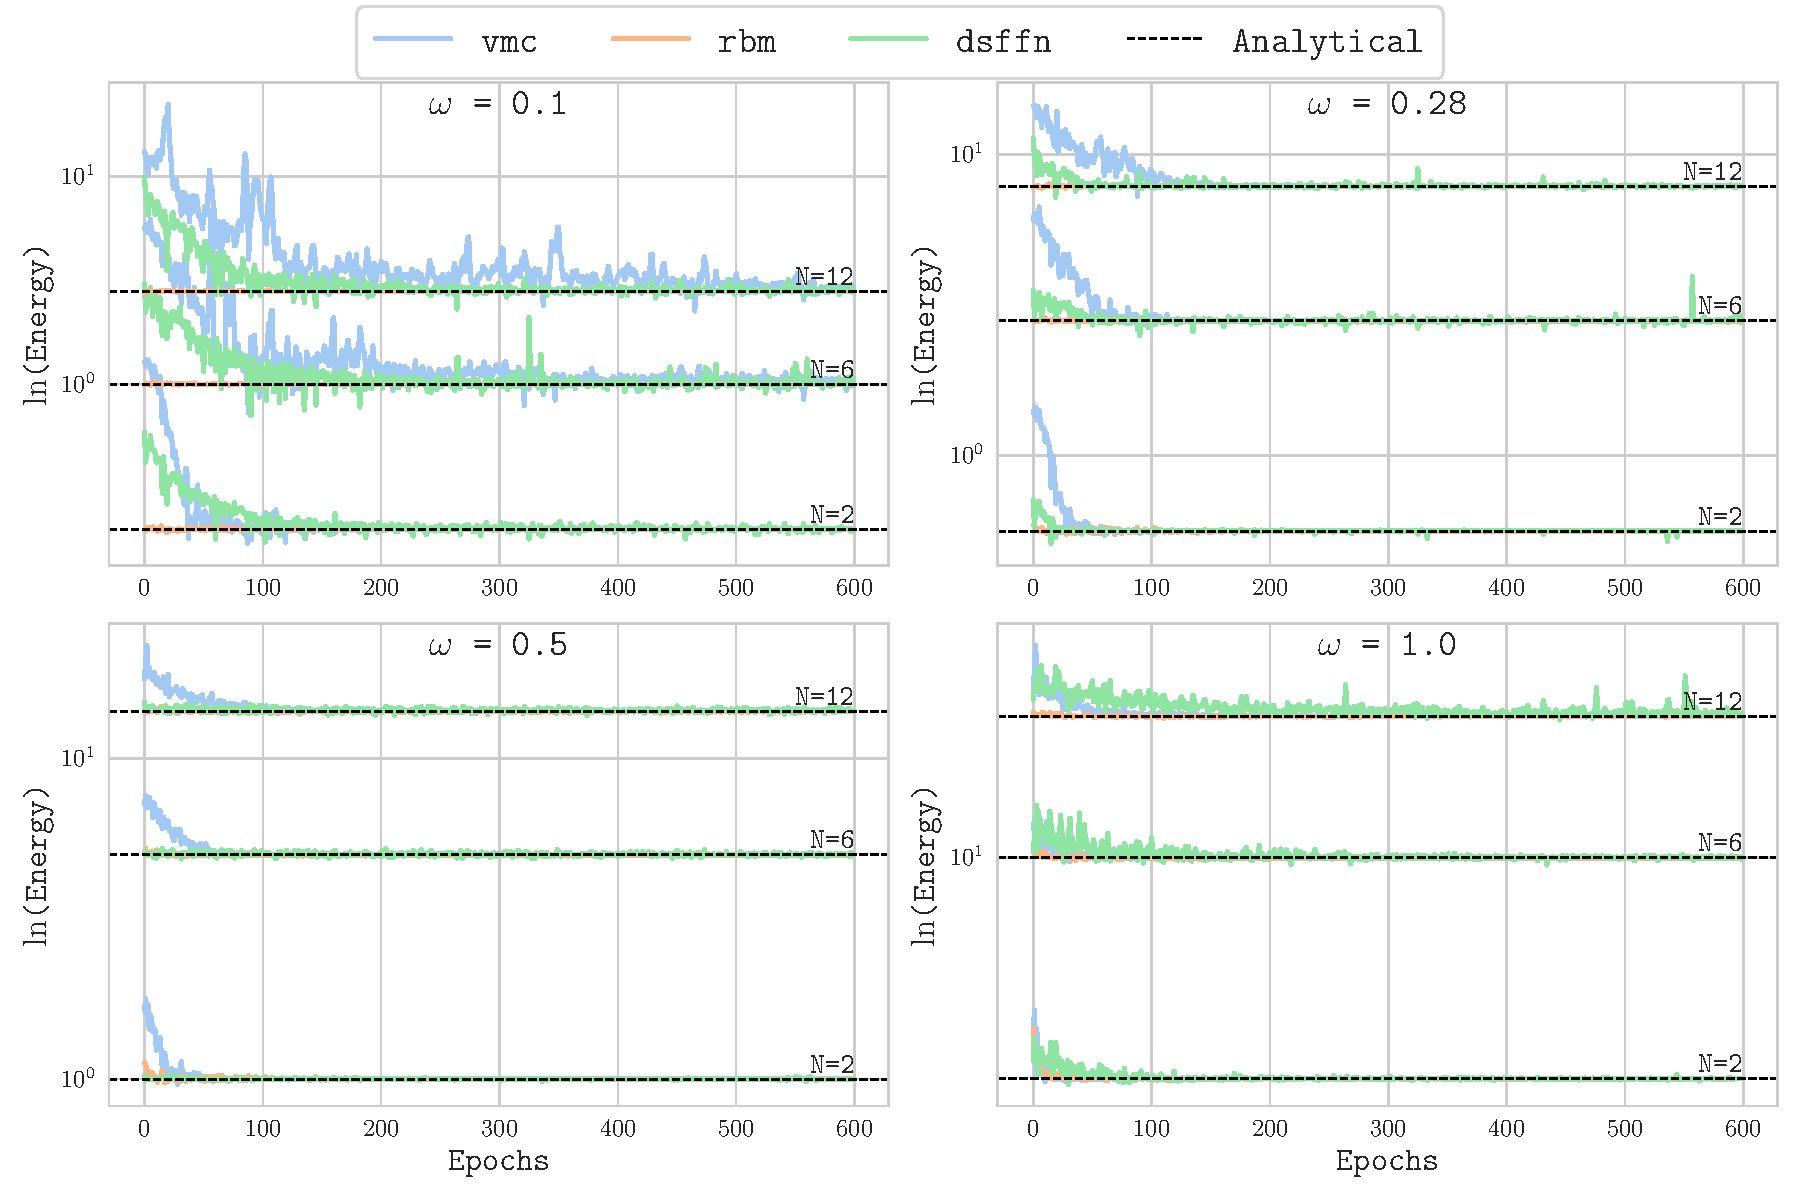
\includegraphics[width=0.9\linewidth]{Chapters/Results/dots/E_conv_ferm_dots_NI.pdf}
    \caption{Logarithmic energy convergence curve for the non-interactive problem of two-dimensional quantum dots. In black dotted line, the analytical ground state energy is marked. The three displayed models are deep set FFN (``dsffn''), restricted Boltzmann machine (``rbm'') and a standard variational Monte Carlo (``vmc''). Except for the Deep Set, Adam optimizer was used. The RBM line is hard to see as the RBM is initialised very close to the analytical solution.}
    \label{fig:E_conv_ferm_pol_NI}
\end{figure}


We again start by showing in \figref{fig:E_conv_ferm_pol_NI} that any of the models can obtain the ground state for different frequencies. We show four values of frequency, which will be used throughout the rest of the study, and we use different models and numbers of particles. Similarly to the case of the non-interacting, one-dimensional spinless fermions, we see that this task is reasonably simple, as no fine-tuning or Jastrow factors were used. We display the energy values on a logarithmic scale for the ease of comparison between energies of systems with different numbers of particles.


\section{Hyperparameter search}\label{sec:parameter_search}

In a manner similar to the one-dimensional scenario, we performed a set of hyperparameter optimisations for each of the four particle numbers tested, as detailed in \ref{met:param_search}. To avoid repetition, the individual results of these configuration sweeps are not shown, but they are comparable to what is presented in \ref{fig:ds_complete_sweep}. Unlike the one-dimensional case, we fixed the batch size at 500 proposals and the training cycles at 400 for these short experiments. The parameters tested included the presence or absence of a pre-training step, the use of the regularised gradual Coulomb interaction scheme, different correlation factors (none, Padé-Jastrow, or Jastrow), optimisers, learning rates, and different latent dimension sizes, when the DSFFN is used. It should also be noted that a frequency of $\omega = 1$ was used for all sweeps at this stage.

\subsection{Optimisers}

\begin{figure}[H]
    \centering
    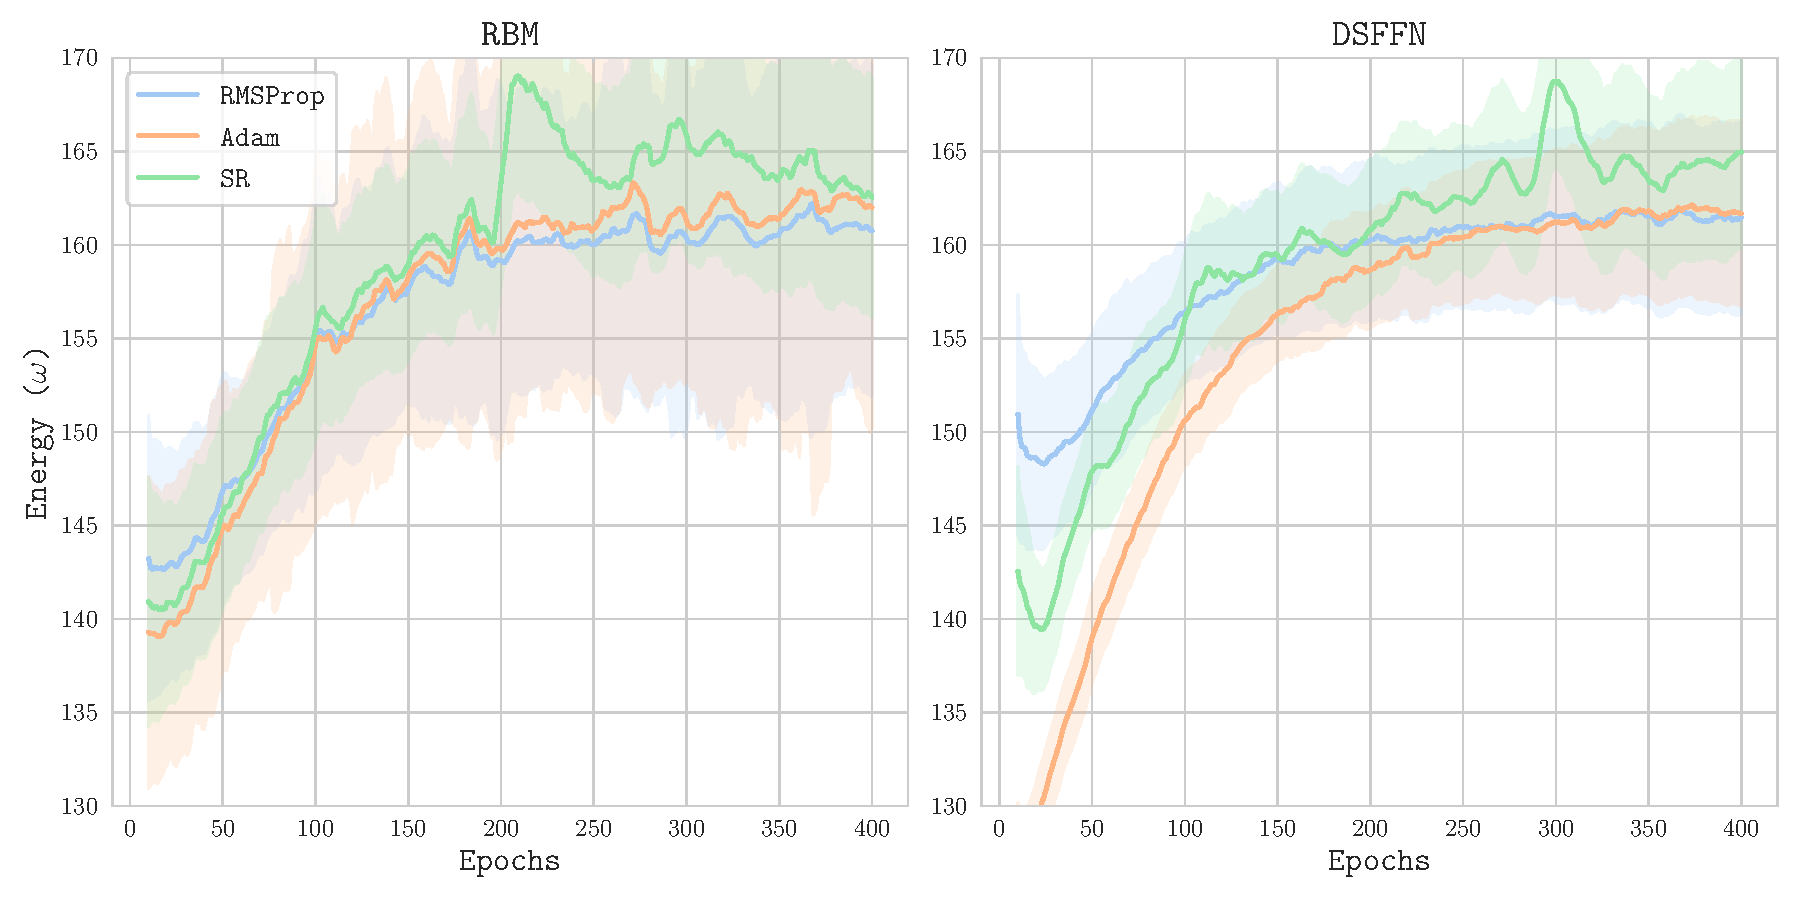
\includegraphics[width=0.9\linewidth]{Chapters/Results/dots/dsffn_vs_rbm_energy_20.pdf}
    \caption{Aggregated values over a Bayesian sweep for 20 particles and frequency of $1.0$. A similar trend is seen for both the RBM and DSFFN. The shaded region is not the error bars, but the minimum an maximum values obtained for over the sweep.}
    \label{fig:dsffn_vs_rbm_energy_20}
\end{figure}


In terms of optimiser choice, we show in \figref{fig:dsffn_vs_rbm_energy_20} the averages of 99 randomly selected parameters for a 20-particle case for the DSSFN ansatz. An analogous behaviour was observed for the two other trial functions. We note that the use of the Bayesian optimisation scheme, explained in \ref{met:param_search}, made the parameter search unbalanced and prevented the choice of stochastic reconfiguration. On that note, for the 20 particle case, SR was chosen 14 times, ADAM 25 and RMSProp was the most frequent, with 60 runs. This was seen for sweeps involving other number of particles as well, and will be further discussed. 

The reason for the infrequent SR choice is that it showed very unpredictable behaviour with respect to the choice of other parameters. When SR managed to converge, it produced good outcomes; however, its variability and often lack of convergence between different configurations were substantial. Then, despite some good individual results, on average RMSProp or Adam were favoured. For this reason, except when showing some selected results, RMSProp was the optimiser of choice for the results to follow.


\subsection{Correlation Factor}

Still investigating the averaged results over random parameters, two analysis can be made with respect to the choice of correlation factor. The following analysis for \figref{fig:corre_std} is done for a 12-particle case for the DSFFN, but the findings were the same for other choices of ansätze and number of particles. Firstly, as indicated in \figref{fig:corre_std}, the absence of any correlation factor resulted in the highest energy values, with the Jastrow factor (``j'' in the figure) producing the lowest energy and the Padé-Jastrow factor (``pj'') having the lowest energy. 

The same can be said with respect to the standard deviation of the energy, further supporting that the Padé-Jastrow factor brings us closer to the ground-state. This indicates that, without correlation factors, even using an ansatz based on parametrised neural networks does not steer us too far from the Hartree-Fock picture, where one single Slater determinant does not enable us to capture significant correlations. 

The lower energy values achieved for the Padé-Jastrow factor is also a positive theory confirmation, as it is supposed to satisfy Kato's cusp condition in a way that is not necessarily the case for the Jastrow factor \cite{huang1998spin}, while also being symmetric under particle exchange.

\begin{figure}[H]
    \centering
    \begin{subfigure}{0.84\textwidth}
        \centering
        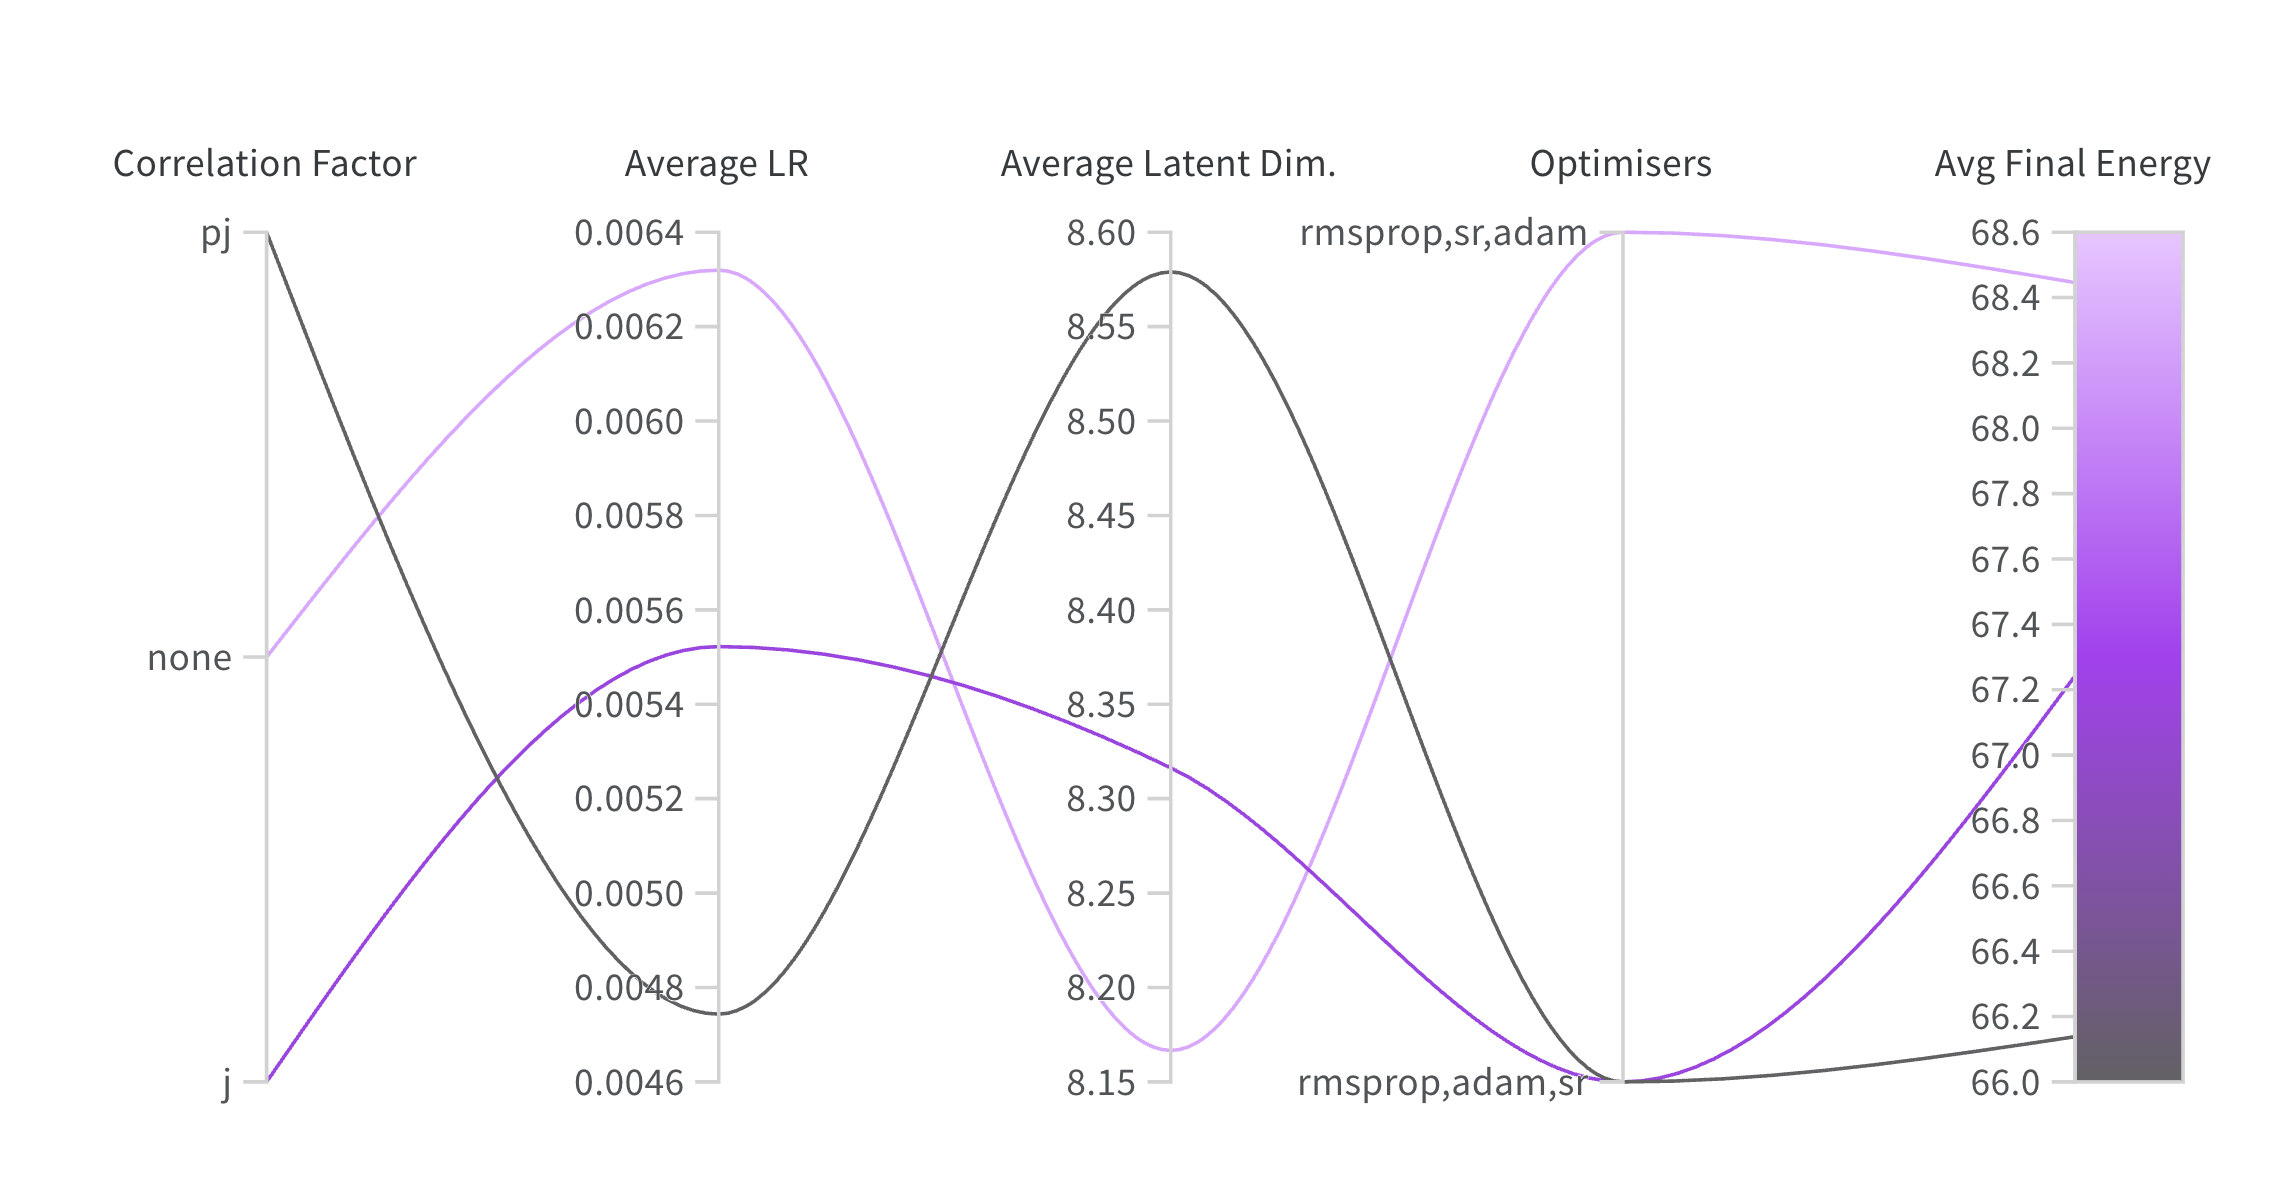
\includegraphics[width=\textwidth]{Chapters/Results/dots/n12_agg_corr.png}
    \end{subfigure}
    \begin{subfigure}{0.8\textwidth}
        \centering
        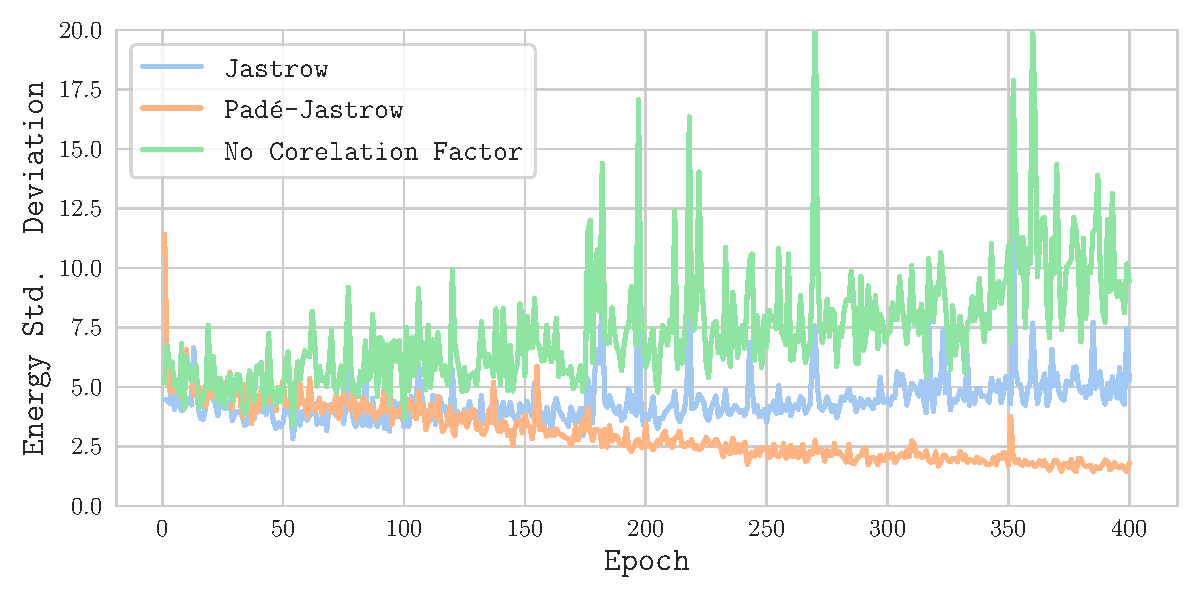
\includegraphics[width=\textwidth]{Chapters/Results/dots/correlation_factorsN_n12.pdf}
    \end{subfigure}
    \caption{Aggregated values over a Bayesian sweep and several parameters (more than what is shown in the parallel line plot) for a 12-particle system and DSFFN trial function. 165 different parameter configuration were performed.}
    \label{fig:corre_std}
\end{figure}

Lastly, an analysis can be performed with respect to the choice of correlation factor. Figure \ref{fig:coulomb_gradual} shows the effect of the correlation factor with the use of a regularised gradual Coulomb interaction potential. Despite these results only being shown for the VMC ansatz and two particles, what is evident is that consistently better results were achieved with both the use of a Padé-Jastrow factor together with the regularised gradual Coulomb interaction. This point is particularly clear when looking at the standard deviations. Although the Padé-Jastrow curve, without the regularised potential, may eventually achieve a lower minimum than the Jastrow curve after the 400 epochs displayed, this occurs much faster with the inclusion of the gradual Coulomb interaction. Again, it is evident that without a correlation factor, the results were sub-optimal in terms of both energy reduction and standard deviation.

Although we do not demonstrate it here, the combination of gradual Coulomb and the Padé-Jastrow factor was also consistently favoured when using the Deep Set network. While nonlinear activation functions theoretically allow the network to capture particle correlations, and this process is further simplified with the regularised gradual Coulomb, the results were better with the combination of these methods than with them in isolation.

\begin{figure}[H]
    \centering
    \begin{subfigure}[b]{0.8\textwidth}
        \centering
        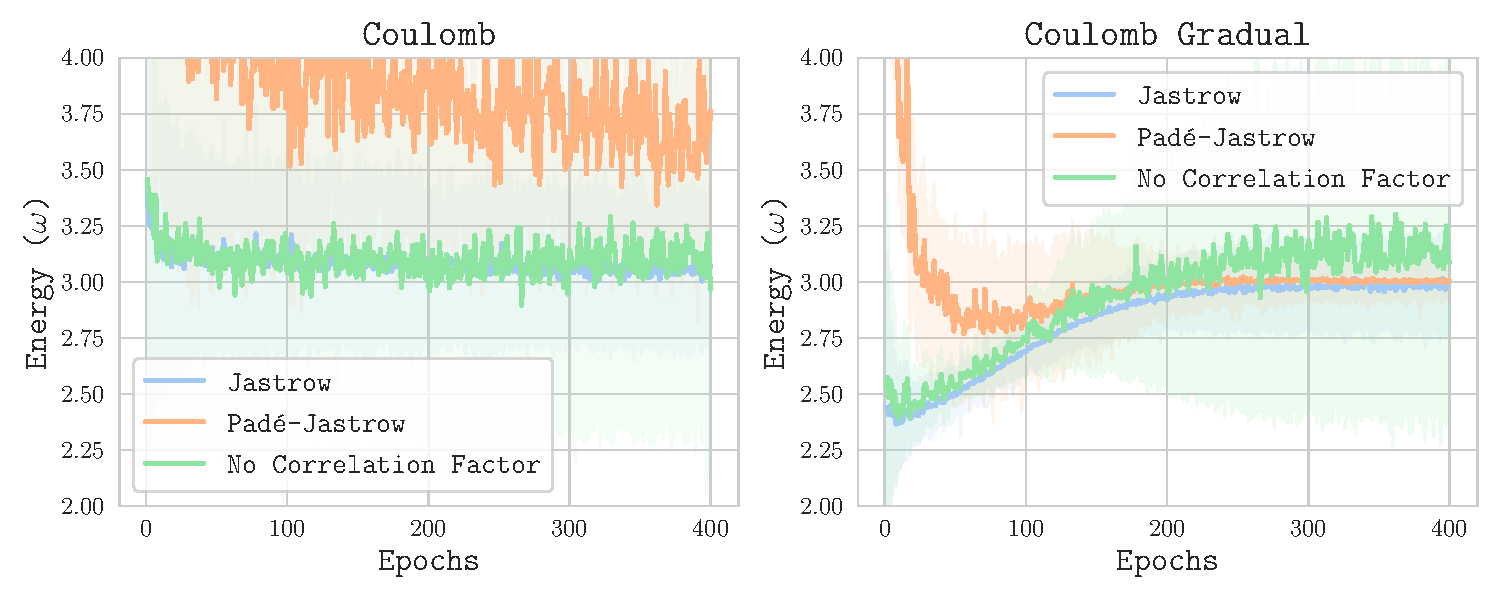
\includegraphics[width=\textwidth]{Chapters/Results/dots/n2_energy.pdf}
        \label{fig:}
        \vspace{-1cm}
    \end{subfigure}
    \begin{subfigure}[b]{0.8\textwidth}
        \centering
        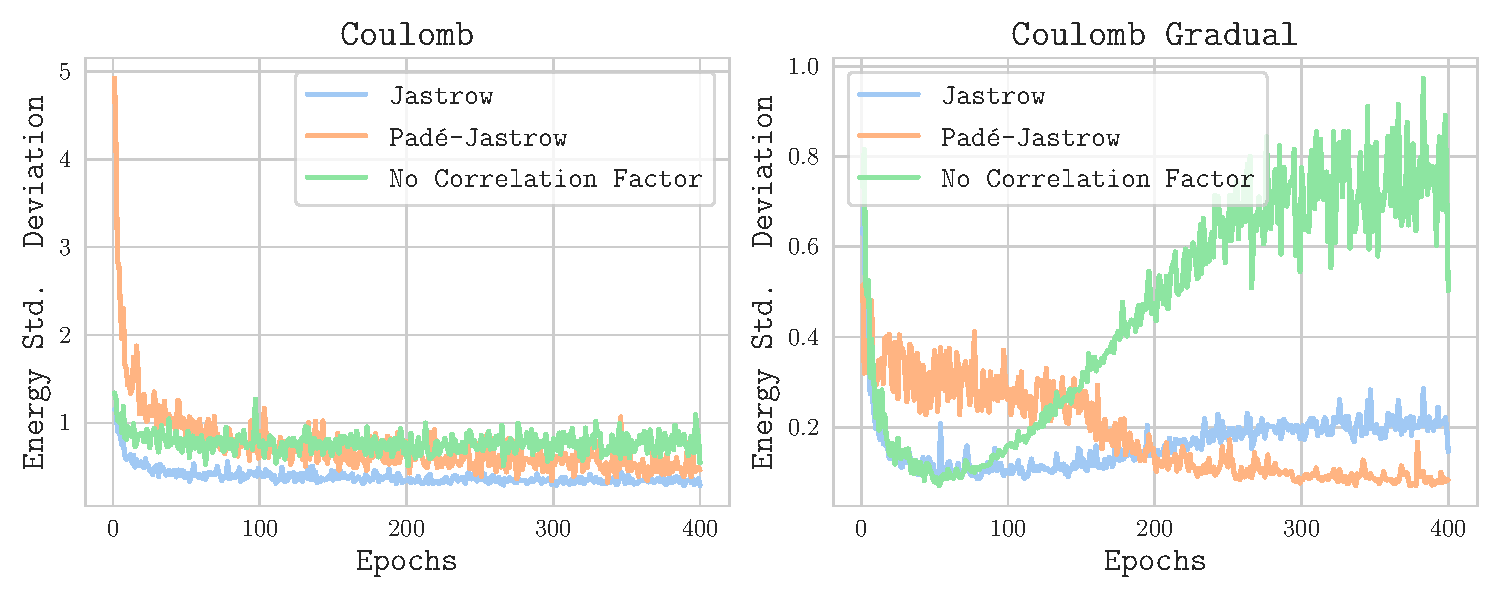
\includegraphics[width=\textwidth]{Chapters/Results/dots/n2_std.pdf}
        \label{fig:}
    \end{subfigure}
    \caption{Aggregated values over a Bayesian sweep and several parameters (see text) for the VMC ansatz and two particle case. Here, a frequency of $\omega = 1$ is selected. The shaded region is not the confidence interval, but the maximum and minimum values obtained from all parameter configurations.}
    \label{fig:coulomb_gradual}
\end{figure}

\section{One and Two-body Densities}

\begin{figure}[H]
    \centering
    \begin{subfigure}[b]{0.82\textwidth}
        \centering
        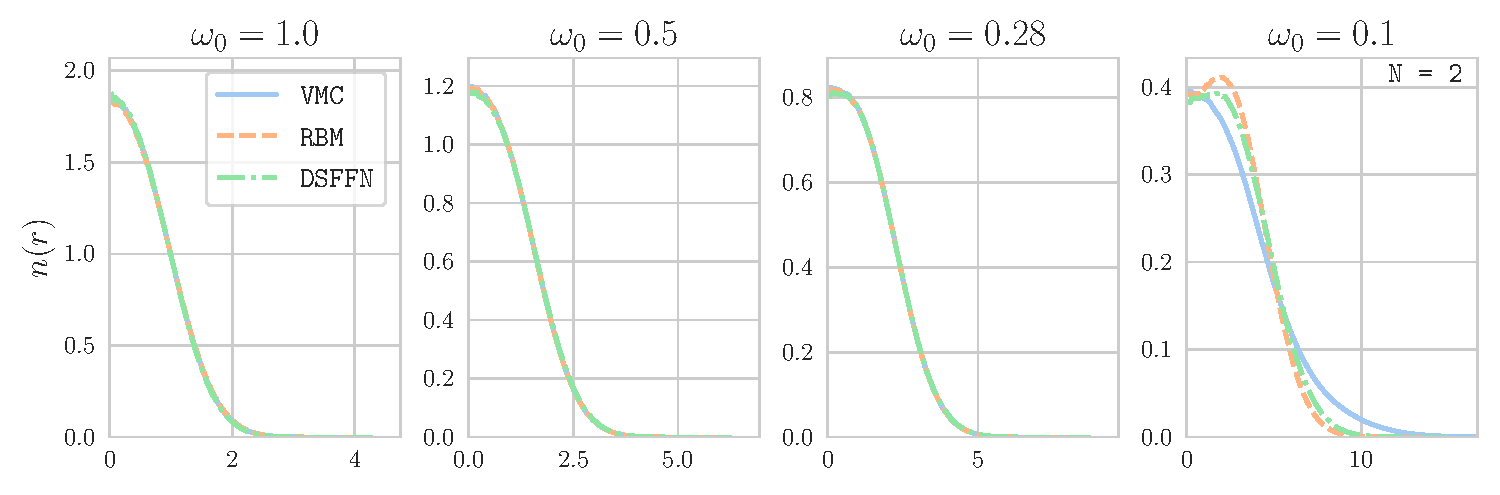
\includegraphics[width=1.0\textwidth]{Chapters/Results/dots/radial_profile_N[2]_nqs_all.pdf}
        \label{fig:total_n2}
        \vspace{-0.4cm}
    \end{subfigure}
    \begin{subfigure}[c]{0.8\textwidth}
        \centering
        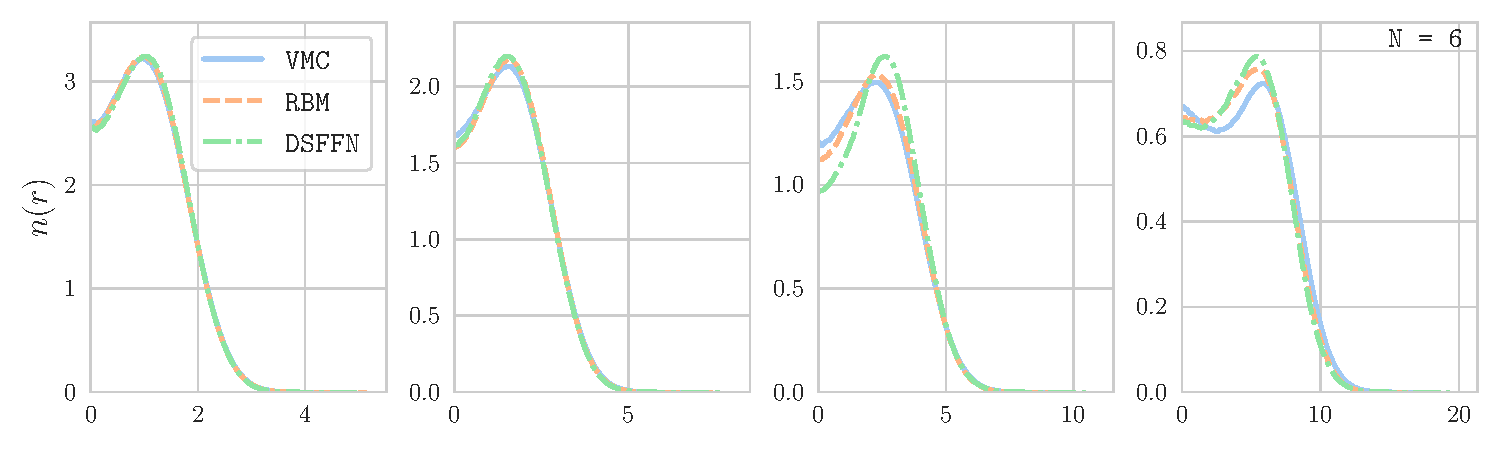
\includegraphics[width=1.0\textwidth]{Chapters/Results/dots/radial_profile_N[6]_nqs_all.pdf}
        \label{fig:total_n2}
        \vspace{-0.4cm}
    \end{subfigure}
    \begin{subfigure}[d]{0.8\textwidth}
        \centering
        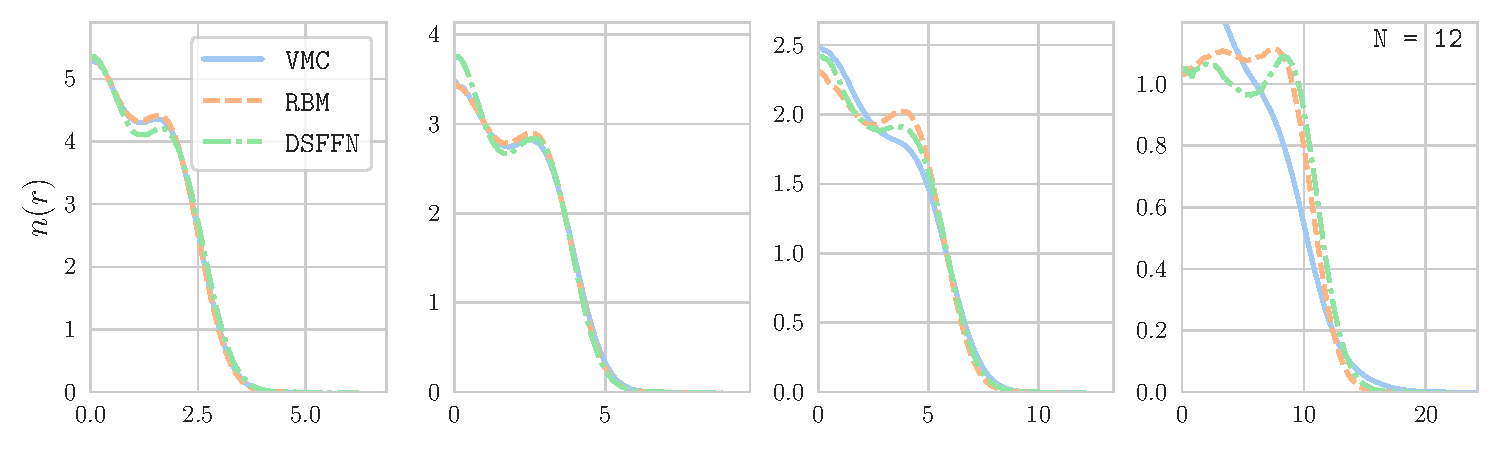
\includegraphics[width=1.0\textwidth]{Chapters/Results/dots/radial_profile_N[12]_nqs_all.pdf}
        \label{fig:total_n4}
        \vspace{-0.4cm}
    \end{subfigure}
    \begin{subfigure}[e]{0.8\textwidth}
        \centering
        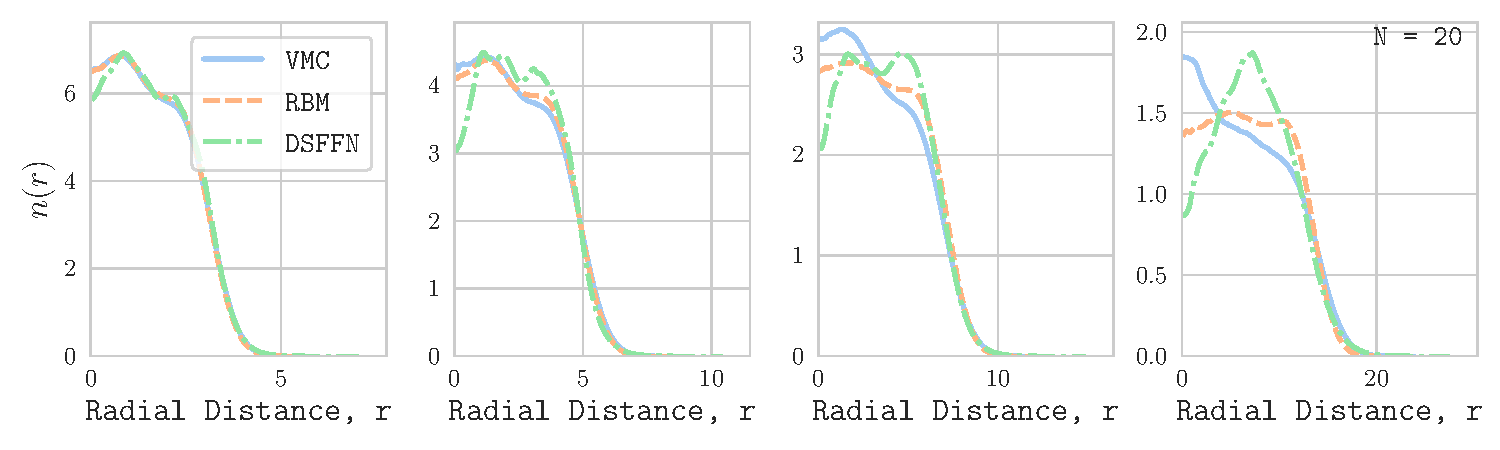
\includegraphics[width=1.0\textwidth]{Chapters/Results/dots/radial_profile_N[20]_nqs_all.pdf}
        \label{fig:total_n6}
    \end{subfigure}
    \caption{Radial density profiles for different ansätze, after $2^{24}$ MC samples. All ansätze were multiplied by a Padé-Jastrow factor, and the sampled energies can be found in Tab. \ref{tab:final_energies}}
    \label{fig:one_body_densities}
\end{figure}


In \figref{fig:one_body_densities}, we display one-body radial densities for up to 20 particles and for different frequencies. A comparison can be made in terms of the different trial functions, but all the models shown contained a Padé-Jastrow factor. It is clear that for higher frequency traps (leftmost in the plots), the radial scale significantly changes. One might overlook the fact that the plots are rescaled for consistent visibility. As expected, for higher frequencies, the particles are more localised and confined closer to the origin. In terms of particle number, again as expected, the profile heights are more pronounced with a larger number of particles, as $n(r)$ integrates to $N$. One sees that a higher density of fermions also induces more peaks in the profile. This is because there is less effective space, yet fermions still have to satisfy the exclusion principle, where fermions must occupy distinct energy levels. Then, the occupation of these levels lead to a shell structure where the fermions are forced to occupy higher energy states which leads to the fringes in the density profile.

For lower-frequency traps, we also know that the quantum energy levels become closer together. This closer spacing directly impacts the character of the fringes in the density profile. Due to the closer spacing of the energy levels, more levels must be populated because of the exclusion principle. This results in a greater number of fringes appearing in the density profile. Nevertheless, these fringes are typically less distinct and more diffuse compared to those in higher frequency traps. Despite the difficulties in capturing correlations for the low-frequency regime, all models in \figref{fig:one_body_densities} seem to replicate this in some way.

For different ansätze, there is generally good agreement for higher frequencies. This is not the case for the inferior right part \figref{fig:one_body_densities}. However, knowing which of the ansatz better represents what is expected is hard only with the density profiles, and this analysis will have to wait until we investigate the energy values.

Although unfortunate, this discrepancy between the profiles for low-frequency and higher number of particles is expected. Lower frequency traps, which are spatially wider, are particularly hard to model when the Coulomb interaction is present. This is due to the long-rage interaction of the Coulomb potential, which follows $1/r$ with $r$ the distance between the particles. Then, even when separated by large distances, the particles still significantly affect each other. This increases the complexity of the correlation, which becomes less localised. This would not be the case, for example, if instead we had a Yukawa potential, which takes the form $\exp(-kr)/r$, with $k$ being a constant. This potential decreases more rapidly as the distance between particles increases.

The exact same analysis that was performed for the radial density profile can also be done for the two-dimensional one-body densities of \figref{fig:3dobd}. We therefore do not repeat it here, but only display the 12 and 20 particle cases for a frequency of $\omega = 1.0$. The two and six particle cases can be seen in the Appendix \ref{apendix:more_results_2d}.

\begin{figure}[H]
    \centering
    % First row of subfigures
    % Second row of subfigures
    \begin{subfigure}[t]{0.32\textwidth}
        \centering
        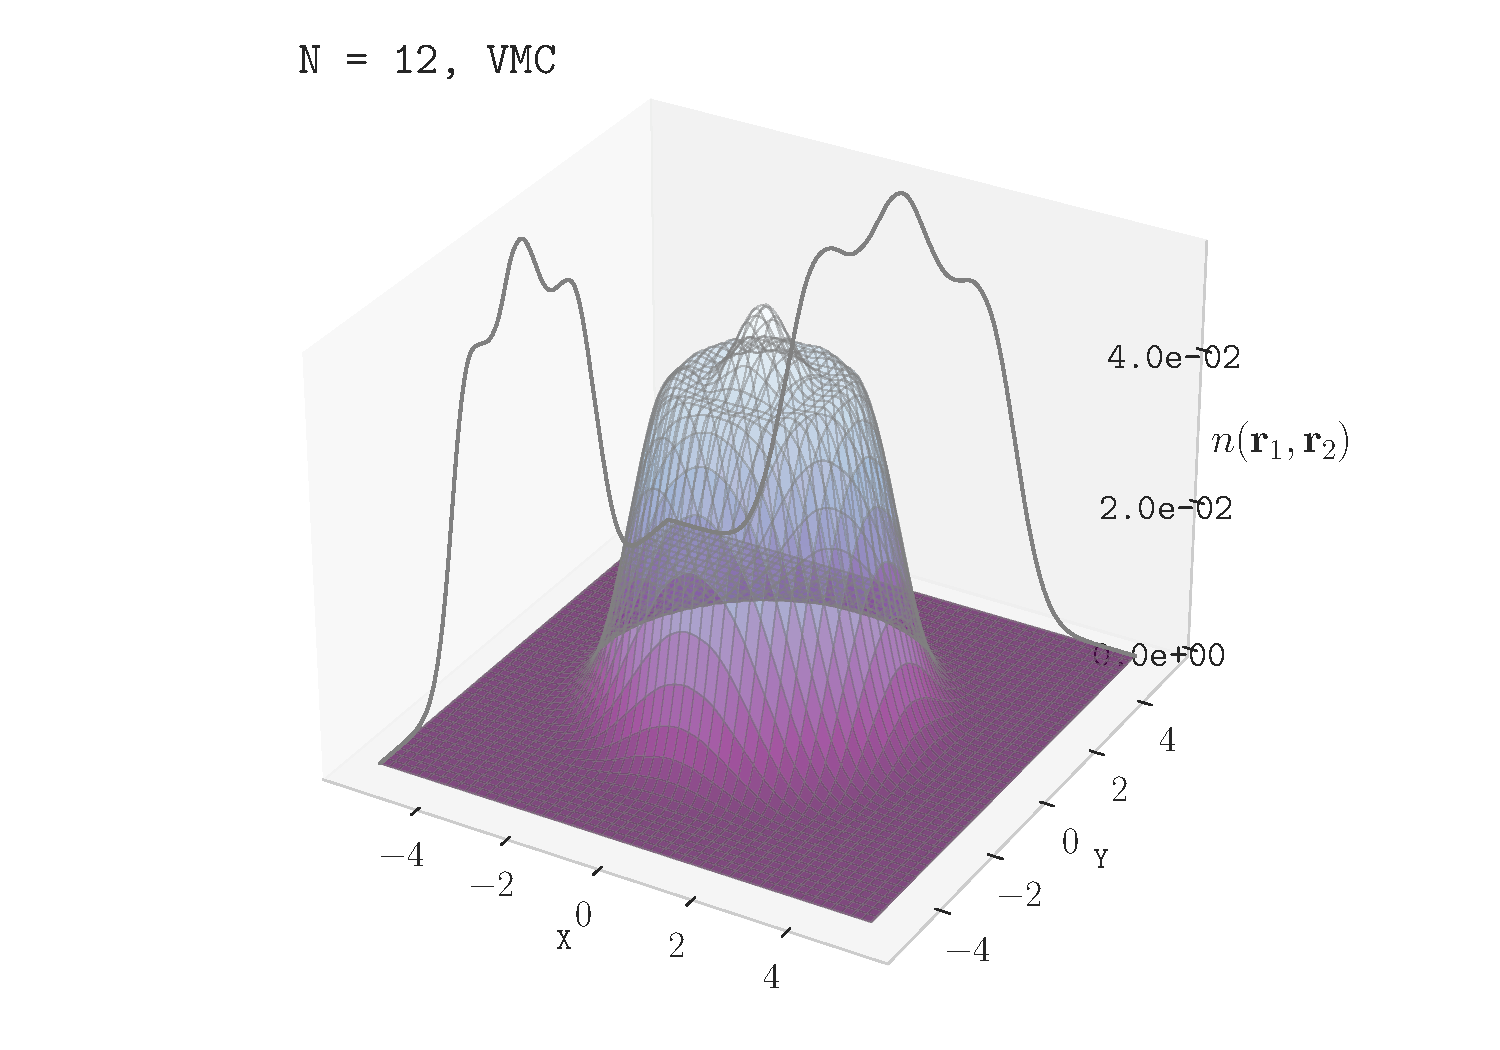
\includegraphics[width=\textwidth]{Chapters/Results/dots/density_profile_3d_N12_nqs_VMC_1.0.pdf}
        \label{fig:sub4}
    \end{subfigure}
    \begin{subfigure}[t]{0.32\textwidth}
        \centering
        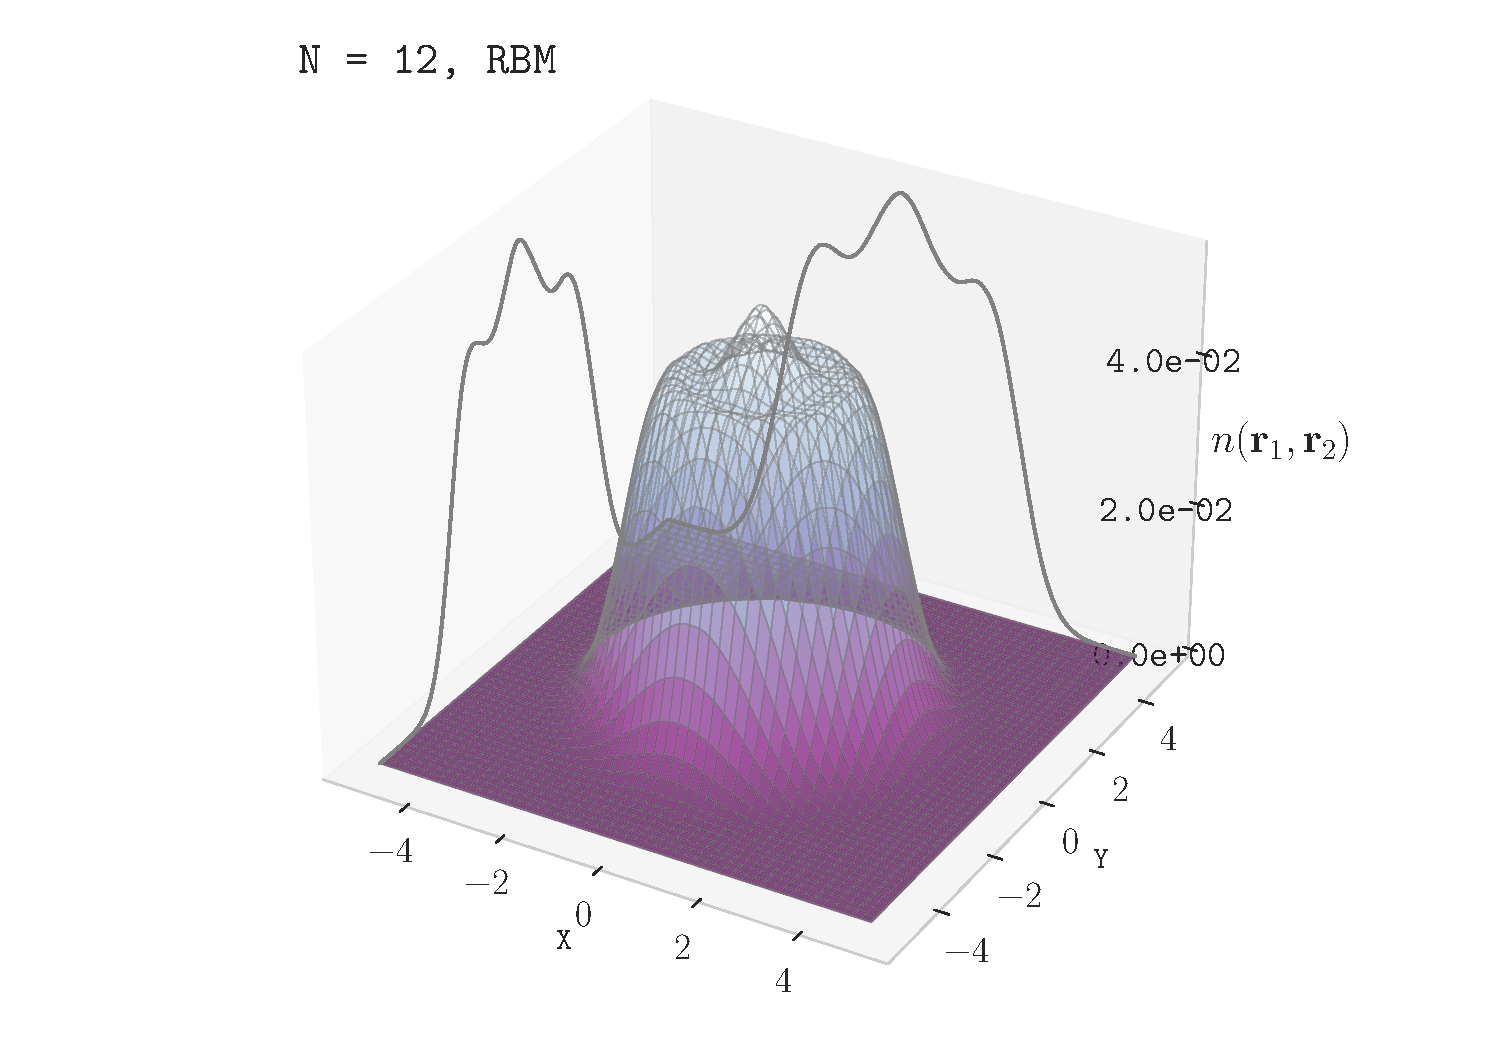
\includegraphics[width=\textwidth]{Chapters/Results/dots/density_profile_3d_N12_nqs_RBM_1.0.pdf}
        \label{fig:sub5}
    \end{subfigure}
    \begin{subfigure}[t]{0.32\textwidth}
        \centering
        \includegraphics[width=\textwidth]{Chapters/Results/dots/density_profile_3d_N12_nqs_dsffn_1.0.pdf}
        \label{fig:sub6}
    \end{subfigure}
    % Third row of subfigures
    \begin{subfigure}[t]{0.32\textwidth}
        \centering
        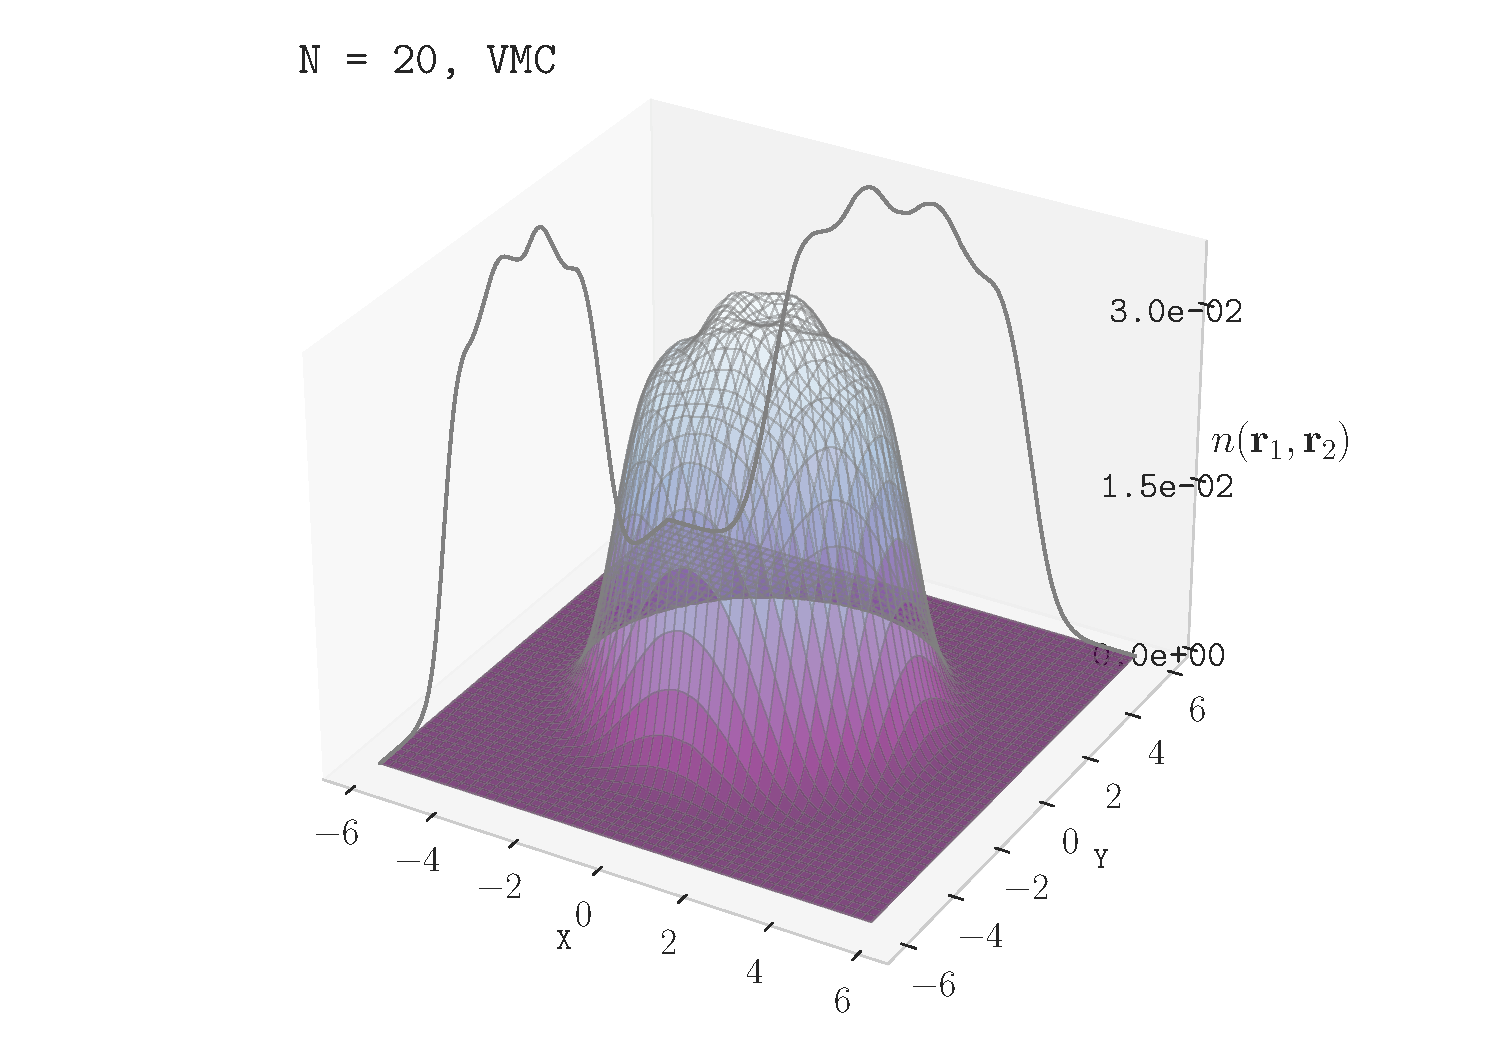
\includegraphics[width=\textwidth]{Chapters/Results/dots/density_profile_3d_N20_nqs_VMC_1.0.pdf}
    \end{subfigure}
    \begin{subfigure}[t]{0.32\textwidth}
        \centering
        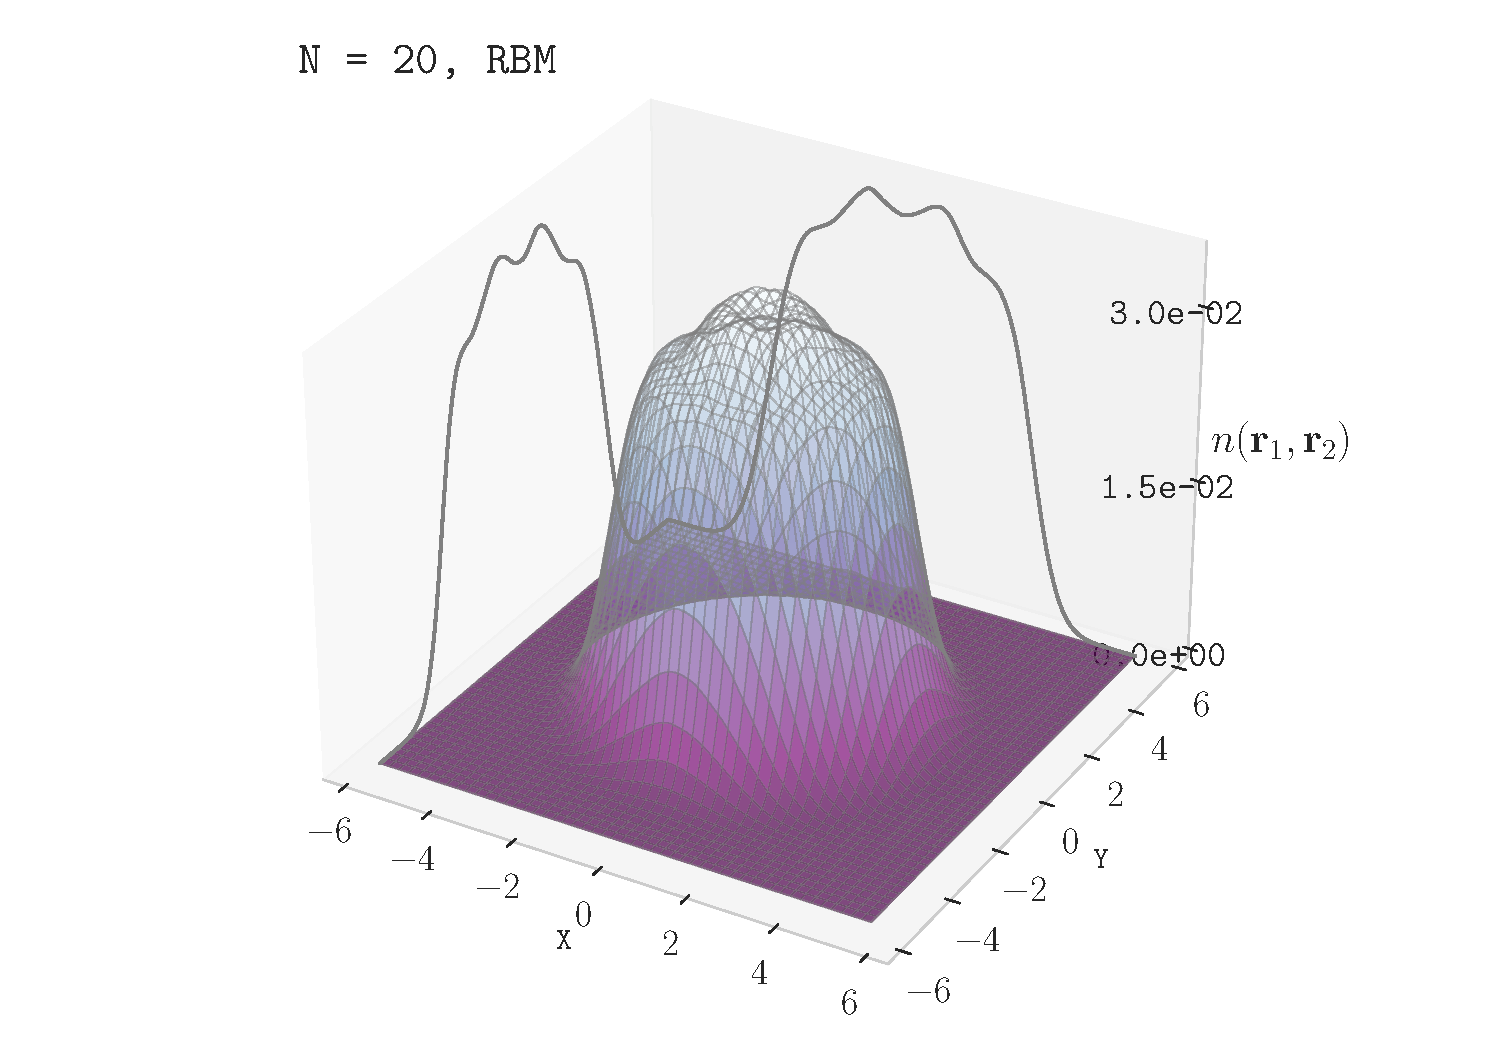
\includegraphics[width=\textwidth]{Chapters/Results/dots/density_profile_3d_N20_nqs_RBM_1.0.pdf}
    \end{subfigure}
    \begin{subfigure}[t]{0.32\textwidth}
        \centering
        \includegraphics[width=\textwidth]{Chapters/Results/dots/density_profile_3d_N20_nqs_dsffn_1.0.pdf}
    \end{subfigure}
    \caption{Two-dimensional one body density profiles for 12 and 20 particles, for all the ansätze used, all of which contained a Jastrow factor. The profiles were made from $2^{24}$ samples, and the final average energies for these can be seen in  Tab. \ref{tab:all_e_final2d}}
    \label{fig:3dobd}
\end{figure}



\begin{figure}[H]
    \centering
    % First row of subfigures
    \begin{subfigure}[t]{0.32\textwidth}
        \centering
        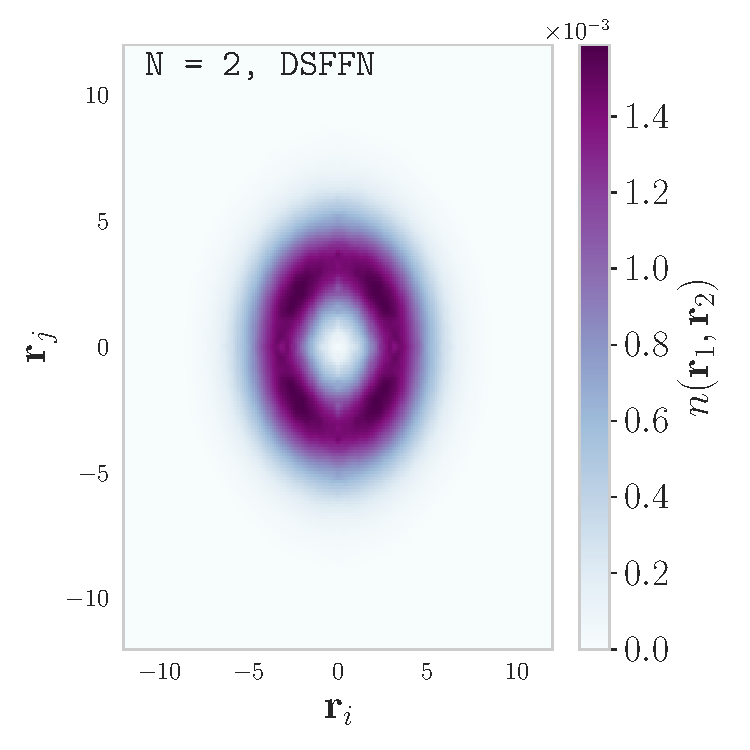
\includegraphics[width=\textwidth]{Chapters/Results/dots/two_body_density_N[2]_nqs_DSFFN_0.1.pdf}
        \label{fig:sub1}
    \end{subfigure}
    \begin{subfigure}[t]{0.32\textwidth}
        \centering
        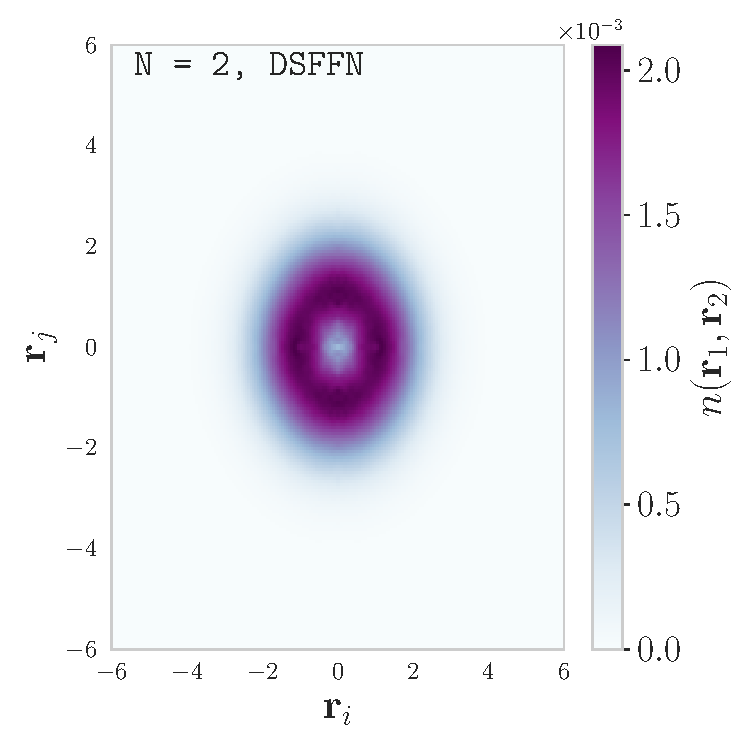
\includegraphics[width=\textwidth]{Chapters/Results/dots/two_body_density_N[2]_nqs_DSFFN_0.5.pdf}
        \label{fig:sub2}
    \end{subfigure}
    \begin{subfigure}[t]{0.32\textwidth}
        \centering
        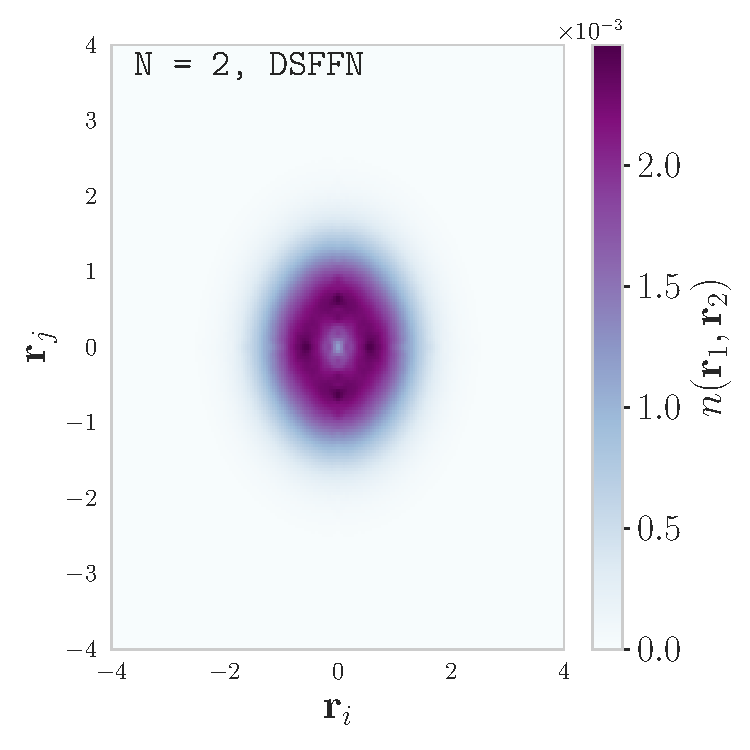
\includegraphics[width=\textwidth]{Chapters/Results/dots/two_body_density_N[2]_nqs_DSFFN_1.0.pdf}
        \label{fig:sub3}
    \end{subfigure}
    \caption{Radial two-body density profiles for the DSFFN ansatz and two particles. From left to right we have frequencies of $\omega = 0.1$, $\omega = 0.5$ and $\omega = 1.0$. The results shown were obtained from $2^{24}$ samples and 3000 training epochs with RMSProp. The densities of the first quadrant were mirrored on the three others to give a symmetric representation.}
    \label{fig:2bdensity2particle}
\end{figure}


Figure \ref{fig:2bdensity2particle} shows that the lower frequency traps, which are wider spatially, also reflect this wider profile in the two-body densities. In fact, pairs of particles are less likely to be seen in the middle of the trap with a lower frequency value. While this figure shows, for the case of two particles, how the density of two bodies changes with frequency, \figref{fig:two_body} shows how the density of two bodies depends both on the number of particles and the choice of ansatz, but now for $\omega = 0.5$.

\begin{figure}[H]
    \centering
    % First row of subfigures
    \begin{subfigure}[t]{0.32\textwidth}
        \centering
        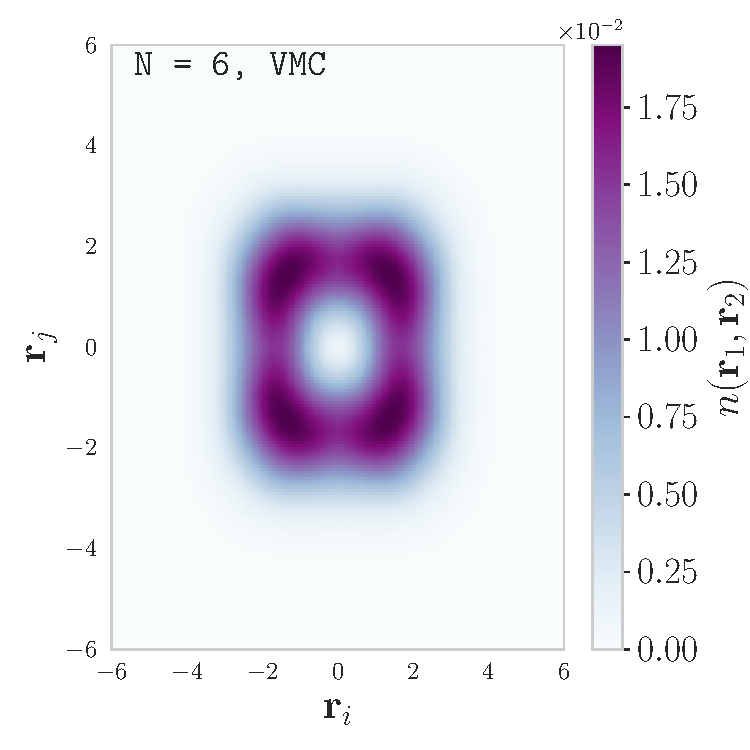
\includegraphics[width=\textwidth]{Chapters/Results/dots/two_body_density_N[6]_nqs_VMC_0.5.pdf}
        \hspace{-1cm}
    \end{subfigure}
    \begin{subfigure}[t]{0.32\textwidth}
        \centering
        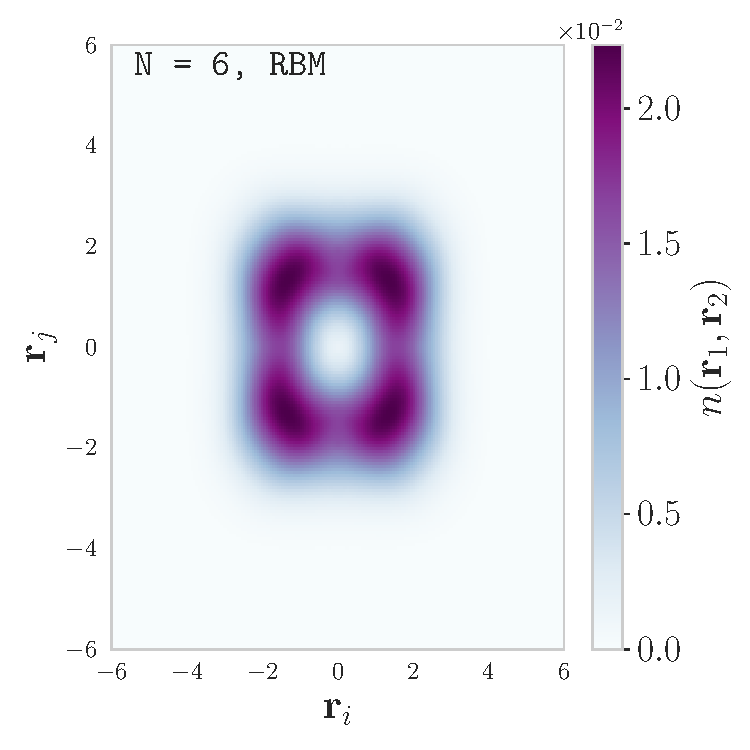
\includegraphics[width=\textwidth]{Chapters/Results/dots/two_body_density_N[6]_nqs_RBM_0.5.pdf}

        \hspace{-1cm}
    \end{subfigure}
    \begin{subfigure}[t]{0.32\textwidth}
        \centering
        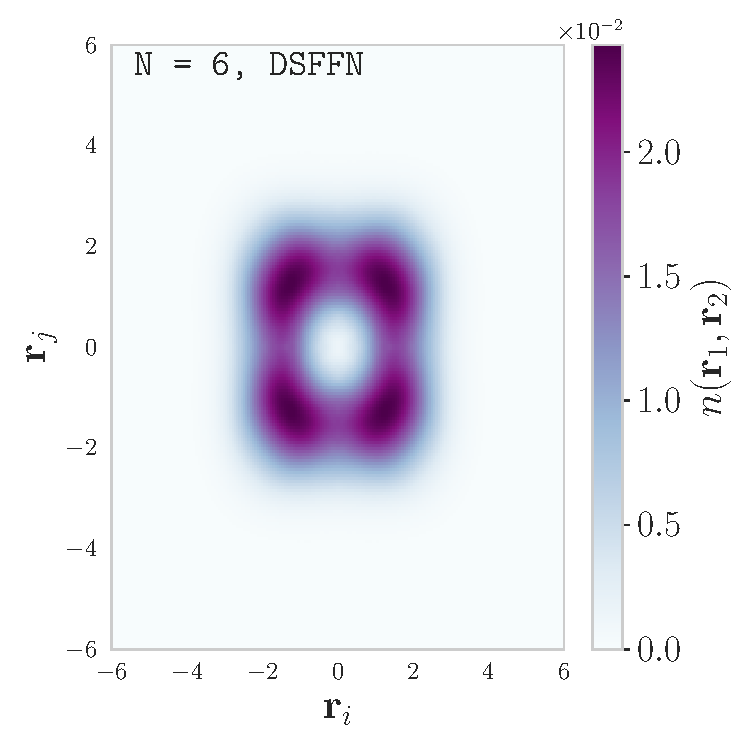
\includegraphics[width=\textwidth]{Chapters/Results/dots/two_body_density_N[6]_nqs_DSFFN_0.5.pdf}
        \hspace{-1cm}
    \end{subfigure}
    % Second row of subfigures
    \begin{subfigure}[t]{0.32\textwidth}
        \centering
        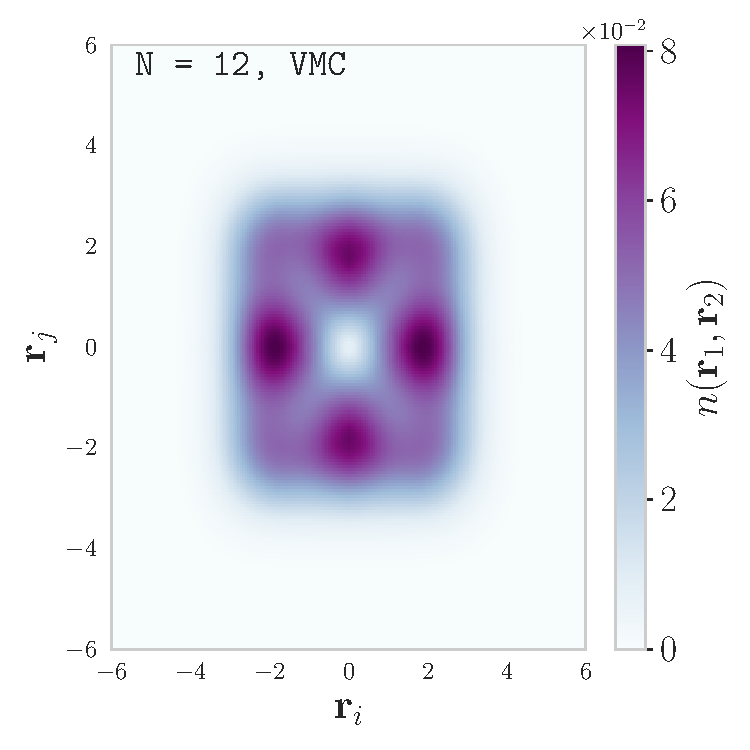
\includegraphics[width=\textwidth]{Chapters/Results/dots/two_body_density_N[12]_nqs_VMC_0.5.pdf}
        \hspace{-1cm}
    \end{subfigure}
    \begin{subfigure}[t]{0.32\textwidth}
        \centering
        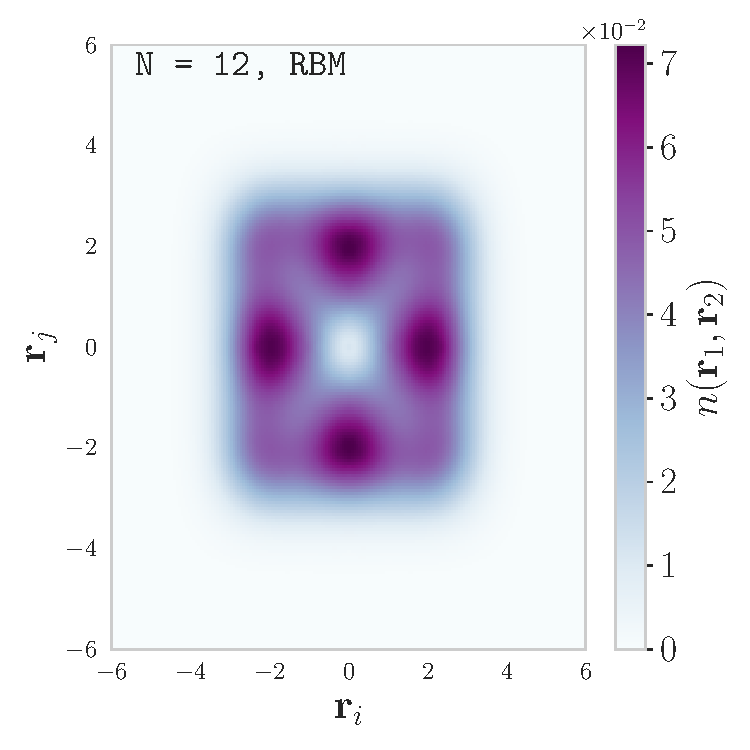
\includegraphics[width=\textwidth]{Chapters/Results/dots/two_body_density_N[12]_nqs_RBM_0.5.pdf}
        \hspace{-1cm}
    \end{subfigure}
    \begin{subfigure}[t]{0.32\textwidth}
        \centering
        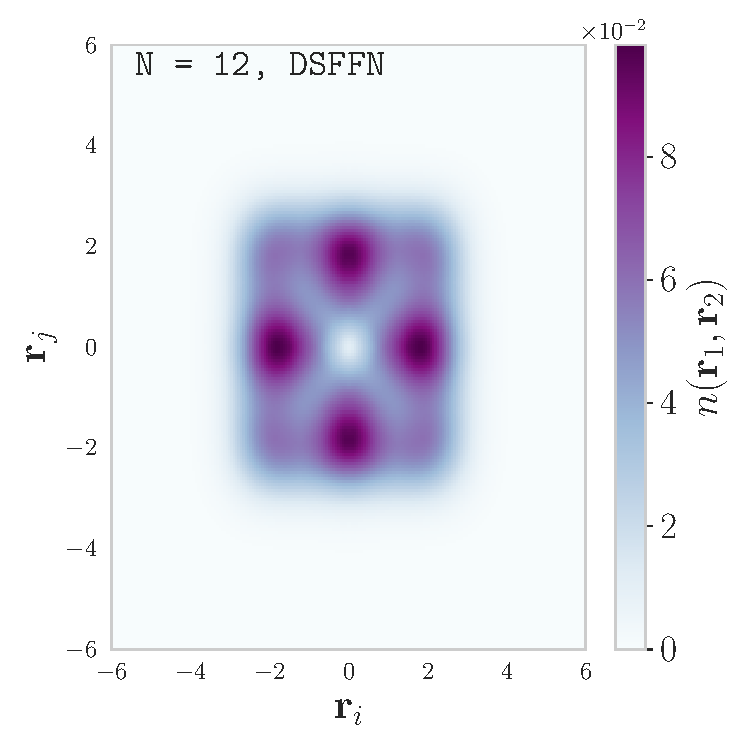
\includegraphics[width=\textwidth]{Chapters/Results/dots/two_body_density_N[12]_nqs_DSFFN_0.5.pdf}
        \hspace{-1cm}
    \end{subfigure}
    % Third row of subfigures
    \begin{subfigure}[t]{0.32\textwidth}
        \centering
        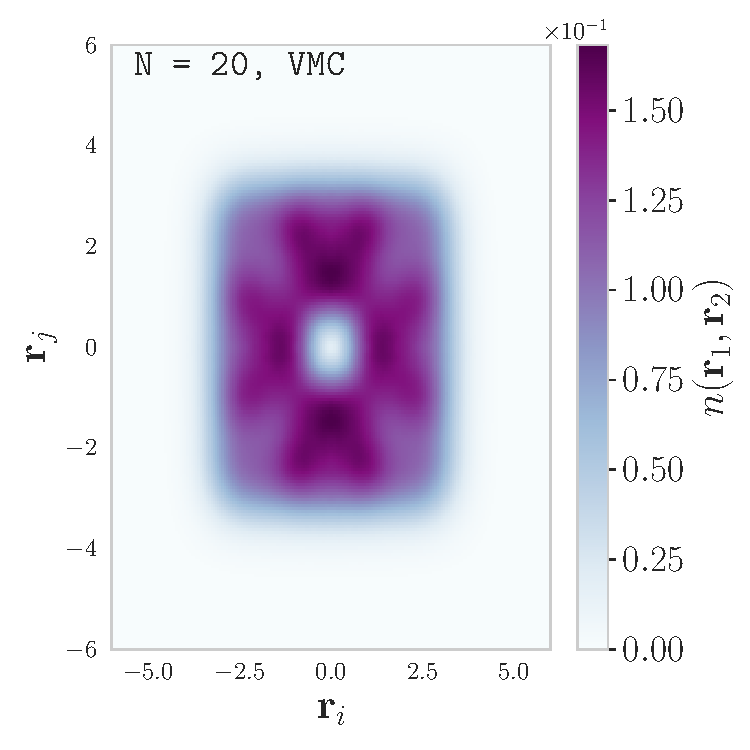
\includegraphics[width=\textwidth]{Chapters/Results/dots/two_body_density_N[20]_nqs_VMC_0.5.pdf}
        \hspace{-1cm}
    \end{subfigure}
    \begin{subfigure}[t]{0.32\textwidth}
        \centering
        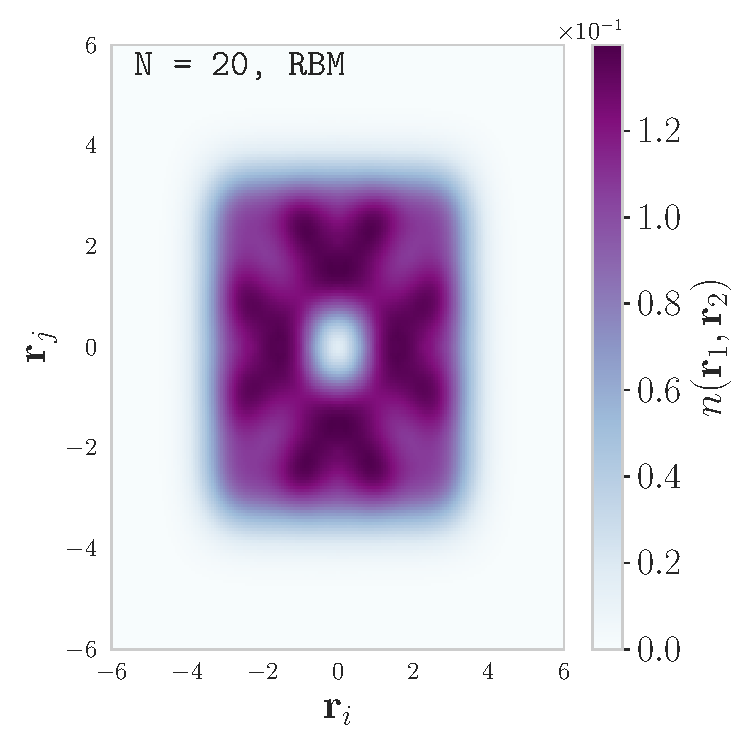
\includegraphics[width=\textwidth]{Chapters/Results/dots/two_body_density_N[20]_nqs_RBM_0.5.pdf}
        \hspace{-1cm}
    \end{subfigure}
    \begin{subfigure}[t]{0.32\textwidth}
        \centering
        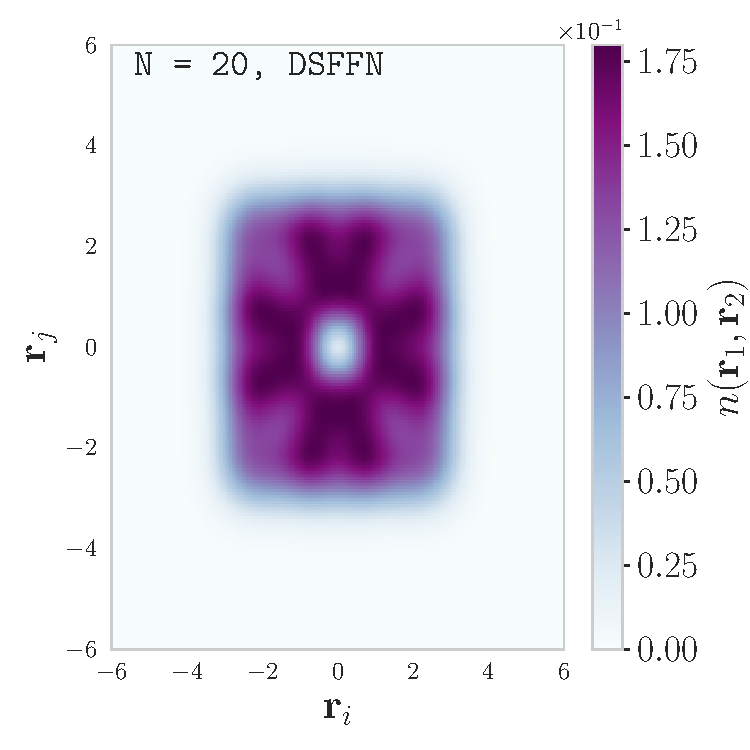
\includegraphics[width=\textwidth]{Chapters/Results/dots/two_body_density_N[20]_nqs_DSFFN_0.5.pdf}
        \hspace{-1cm}
    \end{subfigure}
    \caption{Radial two-body density profiles for $\omega = 0.5$, for all ansätze and different numbers of particles. From top to bottom we have 6, 12 and 20 particles and from left to right we have VMC, RBM and DSFFN. The results shown were obtained from $2^{24}$ samples, trained with 3000 epochs with RMSProp. The densities of the first quadrant were mirrored on the three others to give a symmetric representation.}
    \label{fig:two_body}
\end{figure}

It seems that, from \figref{fig:two_body}, all models are equally capable of capturing approximately the same correlations. The density profiles exhibit a clear symmetry around the origin. Of course, this symmetry was artificially induced by us, in the process of converting the two spatial coordinates into a radial one and replicating the obtained results in the other quadrants. However, this is not an unreasonable procedure, as we see from the one-body density profiles of \figref{fig:one_body_densities} that the position distribution is radially symmetric.

We also notice that pairs of particles prefer to avoid the trap's central region due to their repulsion. As the particle count increases, there is a trend towards the localisation of particle pairs, avoiding the diagonals, which are equidistant from the origin. It appears as though the particles are avoiding the same spatial sphere, which aligns with physical intuition. This pattern is evident with 12 particles, but we observe changes as more particles are added, where they start to avoid not only diagonals but also the principal axes.

\section{Overall Energy Comparison}

\begin{figure}[H]
    \centering
    % First row of subfigures
    \begin{subfigure}{\textwidth}
        \centering
        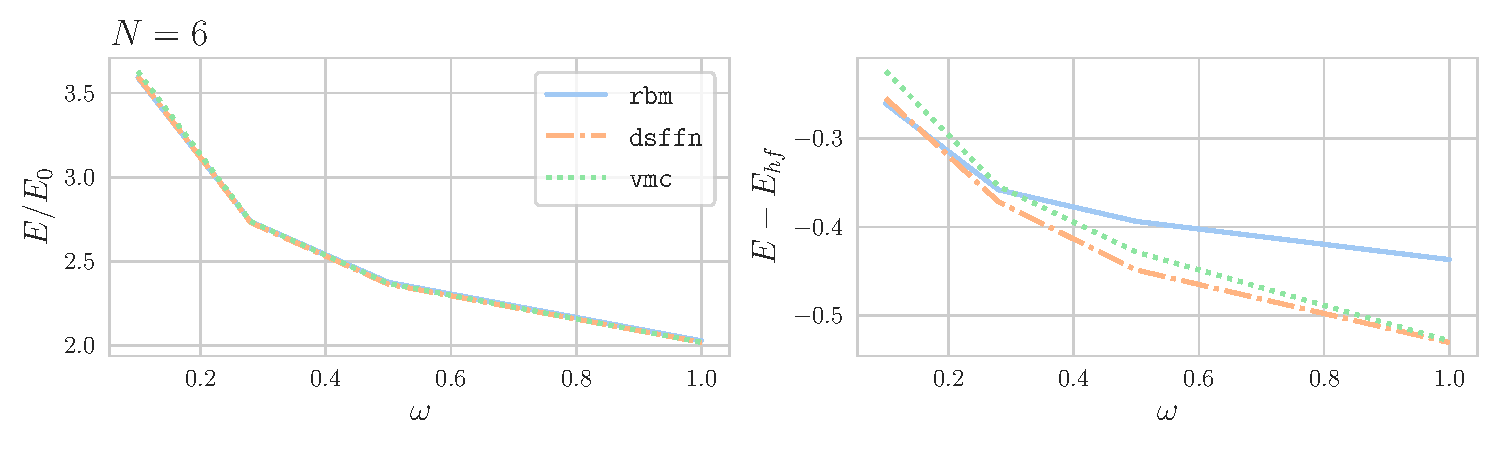
\includegraphics[width=\textwidth]{Chapters/Results/dots/total_energy_vs_omega_n6.pdf}
        \vspace{-1.0cm}
    \end{subfigure}
    \begin{subfigure}{\textwidth}
        \centering
        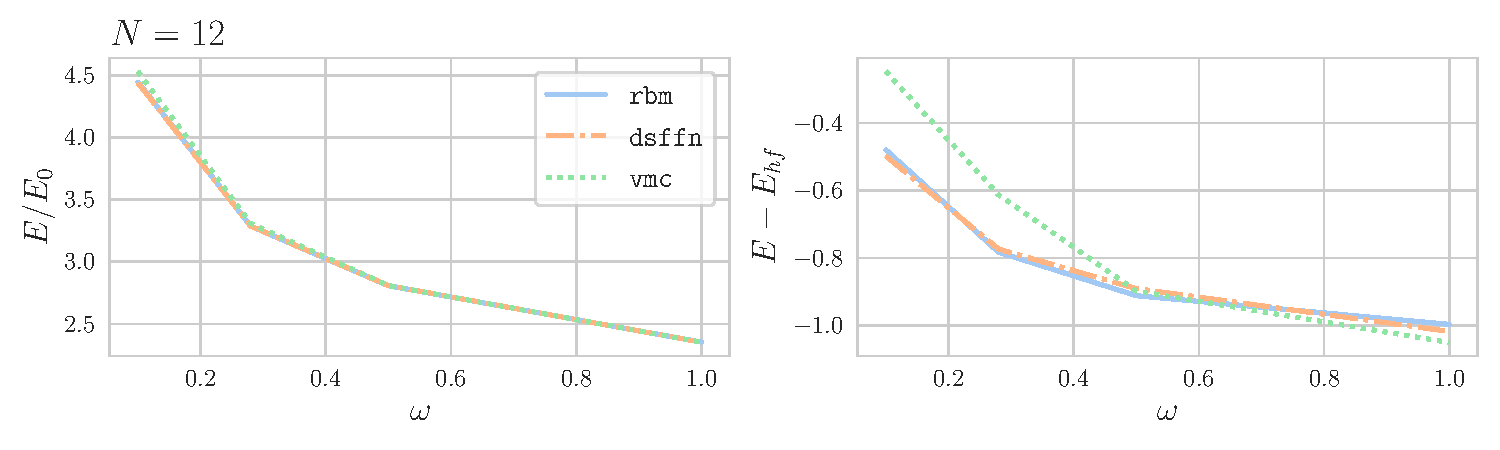
\includegraphics[width=\textwidth]{Chapters/Results/dots/total_energy_vs_omega_n12.pdf}
        \vspace{-1.0cm}
    \end{subfigure}
    % Second row of subfigures
    \begin{subfigure}{\textwidth}
        \centering
        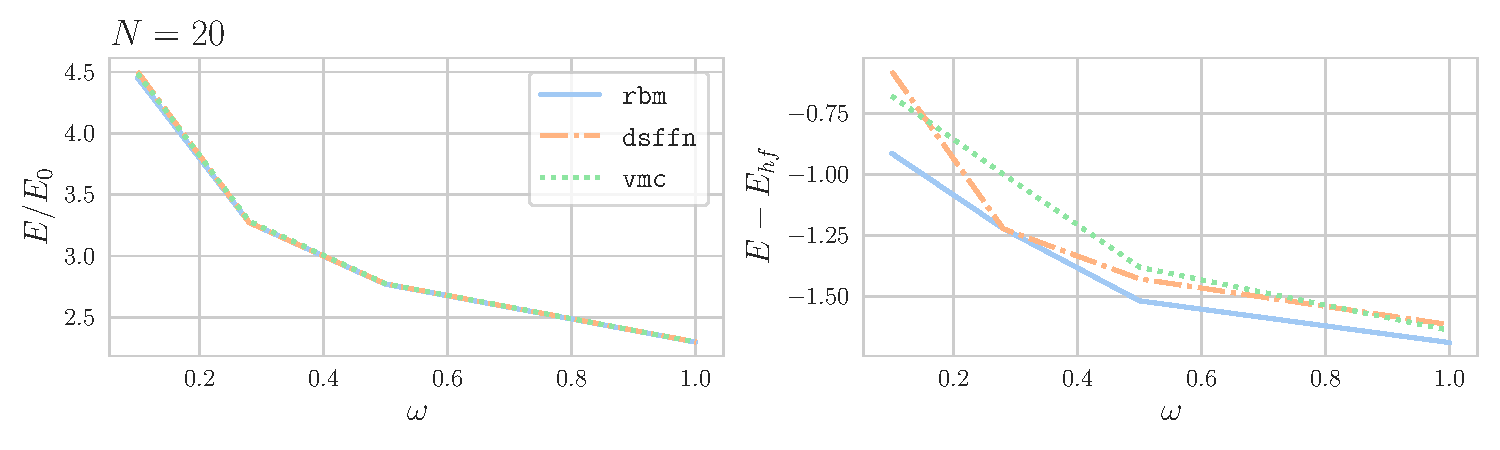
\includegraphics[width=\textwidth]{Chapters/Results/dots/total_energy_vs_omega_n20.pdf}
    \end{subfigure}
    \caption{On the left, the ratio between the measured energy and the non-interactive energy for the same system. On the right, the measure of the correlation energy, $E - E_{hf}$, where $E_{hf}$ is the Hartree-Fock energy value taken from \cite{mariadasonQuantum}. The two-particle case is too similar to the others and is shown in the Apendix \ref{apendix:more_results_2d}}
    \label{fig:correlation_energies}
\end{figure}

The right side of \figref{fig:correlation_energies} is a good reassurance that all our models used achieve energies lower than the HF energy for all ranges of frequencies. These results were gathered after training for 3000 epochs and for $2^{24}$ MC samplings. This is particularly due to the addition of the Jastrow factor in all models at this point. While all models show comparable correlation energies, the RBM model demonstrates exceptionally good performance for the 20-particle case but performs poorly for the six-particle case. The reasons for this discrepancy remain unclear, but it is likely due to sub-optimal hyperparameter choices. Typically, we would anticipate the opposite behaviour.

The fact that \figref{fig:correlation_energies} shows a correlation energy closer to 0 for lower frequency traps further supports our previous discussion about the difficulty of capturing intricate correlations due to the long-range Coulomb interaction. The larger the frequency value, the easier it is for our model to capture correlations that HF is not capable of. %due to the individual single particle Slater Determinant.

The left-hand side of \figref{fig:correlation_energies} shows that as a fraction of the non-interactive energy, all models agree well. The increase in fraction $E/E_0$ with a decrease in frequency aligns with what is found in other studies. As discussed in \cite{kroeze2016trappedelectronsquantumdegenerate}, in fact, this ratio diverges, due to its scaling as $(\omega^{-1/3})$ in the limit of $\omega \to 0$.

Finally, the proportion between energy components can be investigated in \figref{fig:fraction-energies} and in more detail for a six-particle case, in Tab. \ref{tab:fraction_energies}. Naturally, because we are in an interactive regime, the virial theorem is not expected to hold. While there is a distinct trend, a more detailed analysis would require us to investigate beyond the frequency of $1.0$ and below $0.1$. This is because, with the range investigated, we are unable to replicate the expected plateau in the ratio of $\langle K\rangle$ and $\langle V\rangle$ observed in \cite{Nordhagen2019}. The trend we observe at least indicates that with an increase in frequency comes a domination of the kinetic energy term. At low frequencies, the opposite is observed, with potential energy becoming the dominant component of the energy profile, as anticipated. This ratio decreases for larger quantum dots, where the interaction energy increases in proportion as a result of the higher particle count.

\begin{figure}
    \centering
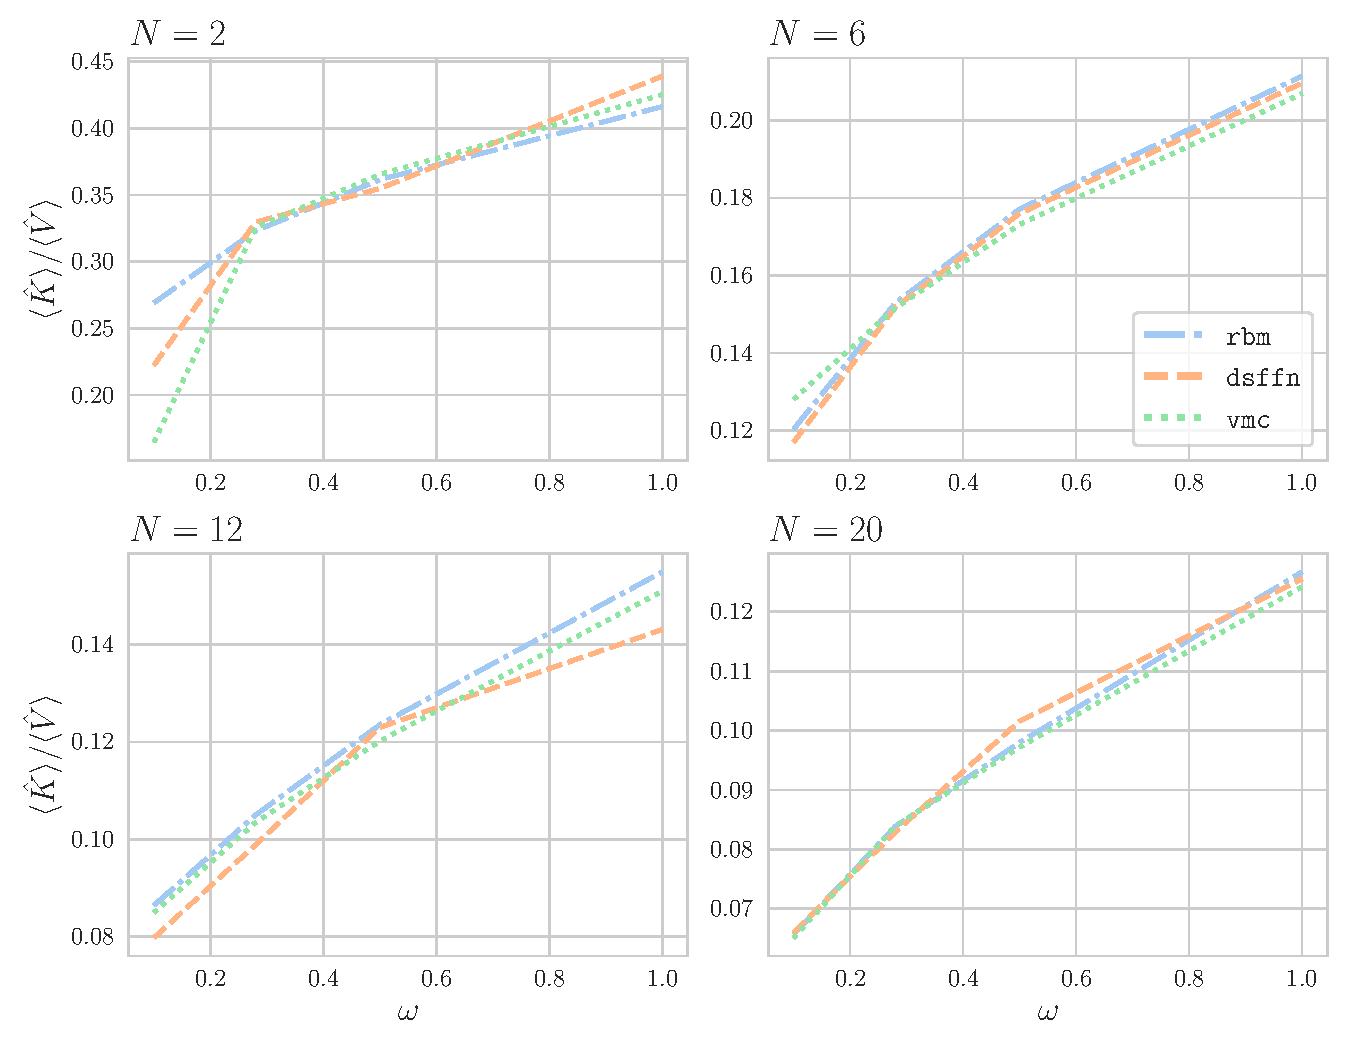
\includegraphics[width=0.8\linewidth]{Chapters/Results/dots/energy_components_vs_omega.pdf}
    \caption{Fraction between kinetic energy and total potential energy as function of the frequency. The total potential energy corresponds to the sum of of interaction energy and the trap energy.}
    \label{fig:fraction-energies}
\end{figure}

\begin{table}[H]
    \centering
\begin{tabular}{c|c|c|c|c|c}
\toprule
\multirow{2}{*}{\textbf{Ansatz}} & \multirow{2}{*}{$\omega$} & \multirow{2}{*}{E} & \multirow{2}{*}{$\langle \hat{K}\rangle$} & \multirow{2}{*}{$\langle \hat{V}_{trap}\rangle$} & \multirow{2}{*}{$\langle \hat{V}_{int}\rangle$} \\
 & & & & & \\
\midrule
\multirow{4}{*}{dsffn} & 0.5 & 11.823(1) & 1.769(3) & 4.261(5) & 5.793(3) \\
 & 1.0 & 20.189(1) & 3.498(5) & 7.651(7) & 9.040(4) \\
 & 0.28 & 7.6481(9) & 1.008(2) & 2.756(4) & 3.884(3) \\
 & 0.1 & 3.5975(7) & 0.377(1) & 1.266(2) & 1.954(2) \\
\midrule
\multirow{4}{*}{rbm} & 0.5 & 11.8778(9) & 1.787(2) & 4.308(4) & 5.782(3) \\
 & 1.0 & 20.2826(8) & 3.539(4) & 7.658(5) & 9.086(3) \\
 & 0.28 & 7.6617(7) & 1.016(2) & 2.702(3) & 3.943(2) \\
& 0.1 & 3.5917(5) & 0.386(1) & 1.292(2) & 1.913(1) \\
\midrule
\multirow{4}{*}{vmc} & 0.5 & 11.8432(8) & 1.748(2) & 4.370(3) & 5.725(2) \\
 & 1.0 & 20.1908(8) & 3.461(4) & 7.727(5) & 9.003(3) \\
 & 0.28 & 7.6657(7) & 1.009(2) & 2.729(2) & 3.928(2) \\
& 0.1 & 3.6281(6) & 0.412(1) & 1.397(2) & 1.819(1) \\
\bottomrule
\end{tabular}
\caption{Energy components from the six particle case for the energy values displayed in \ref{tab:all_e_final2d}.}
\label{tab:fraction_energies}
\end{table}

Lastly, we display in Tab. \ref{tab:all_e_final2d} a collection of the energy values for all models at different frequencies and different numbers of particles. These values were the corresponding values associated to the body densities analysed and all plots other than the ones in the hyperparameter parameter investigation of \ref{sec:parameter_search}. It should be noted that the displayed values result from experiments conducted with a mix of common and unique parameters. Specifically, although all results were achieved after training for 3000 epochs, using RMSProp (except for the SR column), and a batch size of 1000 proposals per epoch, some experiments varied in learning rates and network architectures. This variation was unavoidable, as the scale of the system dictates the architectural choices in several instances, and for larger quantum dots, smaller learning rates were required.

\begin{table}[H]
    \centering
    \begin{tabular}{c|c|cc|c|c|c|c}
    \toprule
    N & $\omega$ & \multicolumn{2}{c|}{\textbf{DSFFN + PJ}} & \textbf{RBM + PJ} & \textbf{VMC + PJ} & \textbf{HF} \cite{mariadasonQuantum} & \textbf{DMC} \cite{hogberget2013quantum} \\
    & & SR & RMSProp & & & & \\
    \midrule
    \multirow{4}{*}{2} & 0.1 & \textbf{0.44146(4)} & 0.4463(2) & 0.44126(3) & 0.545(1) & 0.525635 & 0.44079(1) \\
    & 0.28 &\textbf{1.02218(2)} & 1.02248(4) & 1.02172(1) & 1.02257(3) & 1.14171 & 1.02164(1) \\
    & 0.5 & \textbf{1.66047(6)} & 1.66097(7) & 1.65982(1) & 1.66062129(6) & 1.79974 & 1.65977(1) \\
    & 1.0 & 3.00070(5) & 3.0023(1) & \textbf{3.00009(1)} & 3.00108(5) & 3.16190 & 3.00000(1) \\
    \midrule
    \multirow{4}{*}{6} & 0.1 & & 3.5975(7) & 3.5917(5) & 3.6281(6) & 3.85238 & 3.55385(5) \\
    & 0.28 &\textbf{7.6361(4)} & 7.6481(9) & 7.6617(7) & 7.6657(7) & 8.01957 & 7.60019(6) \\
    & 0.5 & \textbf{11.800(4)} & 11.823(1) & 11.8778(9) & 11.8432(8) & 12.271300 & 11.78484(6) \\
    & 1.0 & \textbf{20.156(7)}& 20.189(1) & 20.2826(8) & 20.1908(8) & 20.719200 & 20.15932(8) \\
    \midrule
    \multirow{4}{*}{12} & 0.1 & & \textbf{12.427(1)} & 12.445(2) & 12.678(3) & 12.9247 & 12.26984(8) \\
    & 0.28 & & 25.776(1) & \textbf{25.767(2)} & 25.937(2) & 26.5500 & 25.63577(9) \\
    & 0.5 & & 39.325(1) & \textbf{39.304(2)} & 39.318(2) & 40.2161 & 39.1596(1) \\
    & 1.0 & & 65.893(1) & 65.914(2) & \textbf{65.860(2)} & 66.9113 & 65.7001(1) \\
    \midrule
    \multirow{4}{*}{20} & 0.1 & & 30.614(4) & \textbf{30.278(3)} & 30.513(4) & 31.1902 & 29.9779(1) \\
    & 0.28 & & \textbf{62.317(2)} & 62.318(5) & 62.541(4) & 63.5390 & 61.9268(1) \\
    & 0.5 & & 94.305(2) & \textbf{94.215(4)} & 94.353(4) & 95.7328 & 93.8752(1) \\
    & 1.0 & & 156.388(3) & \textbf{156.315(4)} & 156.365(4) & 158.004 & 155.8822(1) \\
    \midrule
    \multicolumn{2}{c|}{\textbf{Average}}& & 33.5272 & 33.5058 & 33.6916 & 34.1600 & 33.3523 \\
    \bottomrule
    \end{tabular}
    \caption{Collection of the results for different frequencies and ansätze choices, in comparison to Hartree-Fock and DMC energies. The text in bold font marks the best obtained value for that row. All values were obtained with RMSProp except when shown otherwise. For training, 3000 epochs were used with batch size of 1000. For sampling, $2^{24}$ proposal steps are taken. The missing values for SR mean that we were unable to achieve convergence.}
    \label{tab:all_e_final2d}
\end{table}

All ansätze in \figref{tab:all_e_final2d} showed energy averages lower than Hartree-Fock, but higher than DMC. If we for now disregard the SR column we see that the preferred model was the RBM together with the Padé-Jastrow factor. The DSFFN network was very similar, differing by just $0.02$ on average, while the VMC had the highest energies. 

To address the use of the Stochastic Reconfiguration method, we revisit the topic briefly mentioned in the Bayesian hyperparameter search of \secref{sec:parameter_search}. When this method converged, it demonstrated great results. For instance, at a frequency of $\omega = 1.0$ with six particles, we achieved results superior to those obtained from the DMC calculations. Unfortunately, achieving such a convergence proved to be a challenge. The required parameter choices were unpredictable and lacked intuitive guidance.

One potential explanation is that the neural networks employed were simply too complex models. Although this might be a contributing factor, our experiments with smaller networks did not yield any energy convergence patterns with any of the optimisers tested. Only with more expressive and larger networks did we achieve good results beyond one-dimensional systems.

There might be an unfortunate gap in the complexities of the models tested. A 20-particle VMC ansatz used 40 variational parameters and behaved predictably based on parameter choices. For example, a smaller learning rate generally led to more stable convergence, similar to using a larger batch size. A similar argument applies to the RBM, where changing the number of hidden nodes, sometimes favoured training. An RBM we used for the 20-particle case with 6 hidden nodes displayed 200 parameters, and the Deep Set networks that we used had a similar number. However, we speculate that the non-linear activation layers significantly increased the model's complexity. While this is in general desirable, as we want to be able to capture complex pattern in data, it seems to have made the training process more difficult than expected.

%A final consideration might be made for the fact that none of the models used is guaranteed to be symmetrical or antisymmetric with respect to particle exchange. Even with the guarantee that the Deep Set implementation is sysmmetric, it must be said that the  

\section{Time Scaling Analysis}

Both \figref{fig:time_scalling2d} and Table \ref{tab:time_scalling2d} analyse the wall time scaling for the three models, only for the RMSProp optimiser. The choice of this optimiser was based on its use in presenting nearly all results for this two-dimensional system. Then, while some low-energy values were obtained with SR, we reserve its time scaling discussion for the one-dimensional system, \secref{sec:time_scaling_1d}. Here we analyse the averages over three independent runs for each measurement, with $2^{19}$ sampling steps, up to 22 particles, and for 500 training epochs.

Interestingly, \figref{fig:time_scalling2d} and Tab. \ref{tab:time_scalling2d} seem to indicate very similar polynomial-order scaling for the different trial functions. This affirmation is based on the very close values of $b$ in the polynomial or exponential fits with a constrained constant factor. In \secref{sec:time_scaling_1d} we do a more detailed analysis of how the methods scale with the number of parameters. This analysis suggests that the DSFFN should scale worse than what was measured, and we present some hypotheses as to why this is not the case. 

Firstly, there might be efficient accelerated linear algebra optimisation at play due to the use of just-in-time compilations. More importantly, the choice of architecture size for the DSFFN might have been too small. Here we measure the wall times for the smallest architecture used (architecture one in Tab. \ref{tab:arch}). This was not to be deceptive, but instead a random decision, as we needed to employ varying architectures based on the particle count and frequency to achieve optimal results.

\begin{figure}[H]
    \centering
    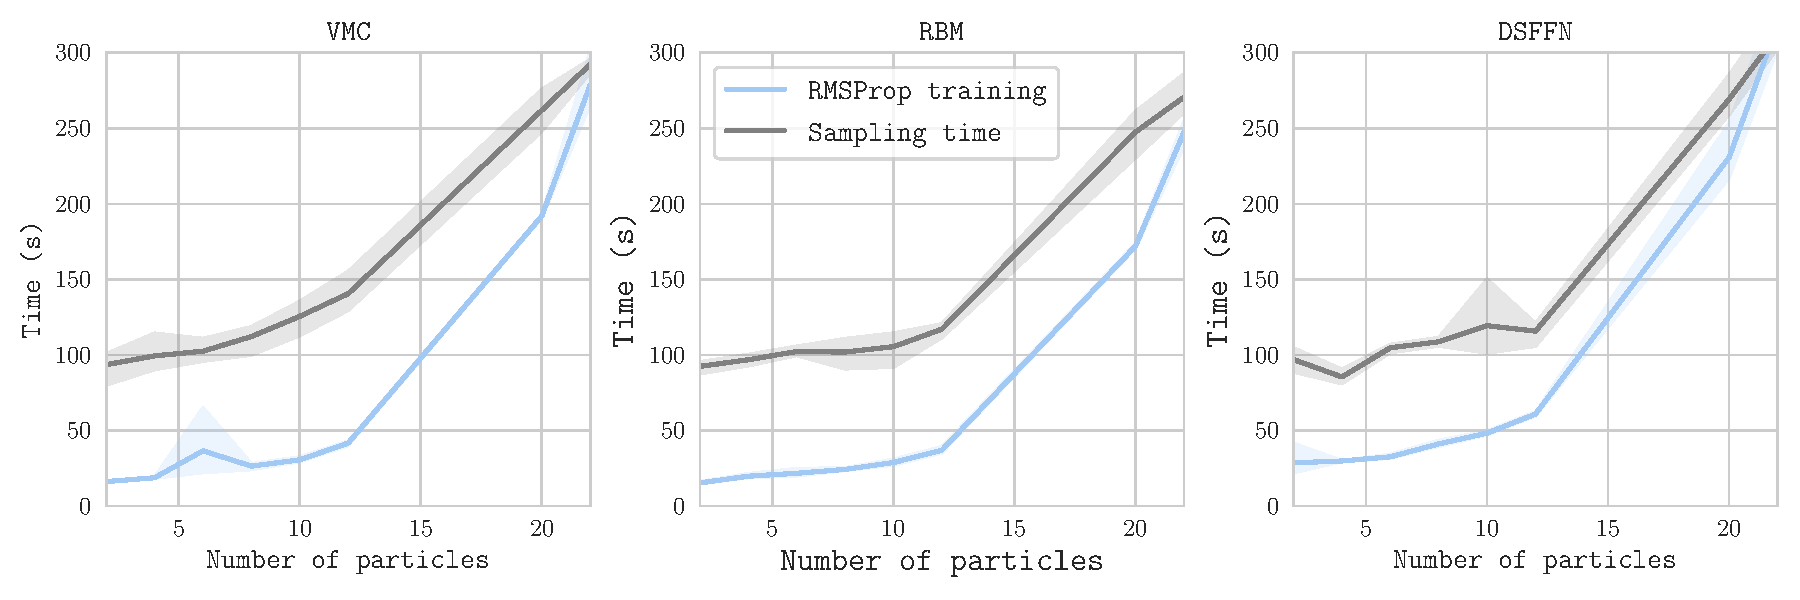
\includegraphics[width=1\linewidth]{Chapters/Results/dots/time_scaling_2d.pdf}
    \caption{Wall time scaling in seconds as a function of number of particles, up to 22 electrons. We display separately the time for sampling and training, where the final wall time is their sum.}
    \label{fig:time_scalling2d}
\end{figure}

For the sake of comparison, it is worth mentioning that we can evaluate our scaling against another study that implemented the same system in C++ \cite{Nordhagen2019}. In their study, they did not use automatic differentiation as we do. For their RBM, under the same constraint of $a=0.5$, they achieved a polynomial degree of approximately $b = 1.5$. This indicates that our scaling is poorer, which is expected given that we are using Python. Nevertheless, our scaling is not significantly worse, and our energy results are comparable.

\begin{table}[h!]
\centering
\caption{Polynomial and exponential fits of time scaling vs. Number of Particles. The leftmost fits do not constrain any coefficients, while the leftmost fits constrains $a = 0.5$.}
\begin{tabular}{llcccccc|cccc}
\toprule
\textbf{Ansatz} & \textbf{Opt.} & \multicolumn{3}{c}{\textbf{Poly.} $(aN^b)$} & \multicolumn{3}{c}{\textbf{Exp.} $(ae^ {Nb})$} & \multicolumn{2}{c}{\textbf{Poly.} $(0.5N^b)$} & \multicolumn{2}{c}{\textbf{Exp.} $(0.5e^ {Nb})$} \\
\cmidrule(lr){3-5} \cmidrule(lr){6-8} \cmidrule(lr){9-10} \cmidrule(lr){11-12}
& & \textbf{a} & \textbf{b} & \textbf{R\textsuperscript{2}} & \textbf{a} & \textbf{b} & \textbf{R\textsuperscript{2}} & \textbf{b} & \textbf{R\textsuperscript{2}} & \textbf{b} & \textbf{R\textsuperscript{2}} \\
\midrule
VMC & RMSProp & 0.05 & 2.76 & 0.96 & 6.60 & 0.17 & 0.98 & 2.02 & 0.94 & 0.29 & 0.93 \\
\midrule
RBM & RMSProp & 0.04 & 2.78 & 0.98 & 5.70 & 0.17 & 0.99 & 1.98 & 0.96 & 0.28 & 0.94 \\
\midrule
DSFFN & RMSProp & 0.24 & 2.32 & 0.97 & 11.68 & 0.15 & 0.99 & 2.07 & 0.96 & 0.30 & 0.89 \\
\bottomrule
\end{tabular}
\label{tab:time_scalling2d}
\end{table}